\chapter{Levítico}

\section*{Introducción al Libro de Levítico}

El \textbf{Levítico} es el tercer libro del \textbf{Antiguo Testamento} y del Pentateuco. Su nombre proviene de la tribu de Leví, de la cual surgieron los sacerdotes encargados de las funciones litúrgicas y el culto en Israel. Este libro se centra en las leyes y rituales que regulan la relación entre Dios y su pueblo, subrayando la santidad como el valor fundamental de la vida en comunidad.

\subsection*{Autoría}

La tradición judía y cristiana atribuyen la autoría de Levítico a \textbf{Moisés}, como parte del Pentateuco. Según esta tradición, Moisés habría recibido las leyes contenidas en el libro directamente de Dios durante su estancia en el Monte Sinaí. Sin embargo, estudios críticos modernos sugieren que Levítico forma parte de la fuente sacerdotal (\textit{P}), redactada durante el período del exilio babilónico (siglo VI a.C.), cuando se buscaba codificar las leyes religiosas para preservar la identidad del pueblo judío.

\subsection*{Temática}

El Levítico aborda principalmente leyes rituales, éticas y de pureza, estructuradas en torno a la idea central de la santidad. Sus temas clave incluyen:
\begin{itemize}
	\item \textbf{Leyes sobre los sacrificios} (Levítico 1–7): Detalla los diferentes tipos de sacrificios, como holocaustos, ofrendas de paz y ofrendas por el pecado, y su propósito en la adoración a Dios.
	\item \textbf{Consagración del sacerdocio} (Levítico 8–10): Relata la ordenación de Aarón y sus hijos como sacerdotes, destacando su papel en el culto.
	\item \textbf{Leyes de pureza} (Levítico 11–15): Regulan aspectos de la vida cotidiana, como los alimentos permitidos, la pureza ritual y la limpieza física.
	\item \textbf{El Día de la Expiación} (Levítico 16): Describe el rito anual para purificar al pueblo y al santuario mediante sacrificios expiatorios.
	\item \textbf{El Código de Santidad} (Levítico 17–26): Contiene leyes morales, sociales y religiosas que llaman al pueblo a vivir en santidad, incluyendo la célebre máxima: “Seréis santos, porque yo, el Señor vuestro Dios, soy santo” (Levítico 19:2).
\end{itemize}



El Levítico refleja la necesidad de establecer un sistema religioso y ético que consolidara la identidad de Israel como pueblo elegido. En el contexto histórico, este libro probablemente fue desarrollado en una época en la que el culto y las leyes religiosas eran fundamentales para mantener la cohesión comunitaria, especialmente durante y después del exilio babilónico.

El énfasis en la santidad, tanto en los rituales como en la vida cotidiana, distingue al Levítico de otros códigos legales de la antigüedad, como el Código de Hammurabi o las leyes hititas. Además, subraya la idea de que la santidad abarca todos los aspectos de la vida, desde la adoración a Dios hasta las relaciones interpersonales.



El Levítico es un manual de santidad que no solo regula el culto, sino también la vida moral y comunitaria del pueblo de Israel. Aunque puede parecer distante para los lectores modernos, su énfasis en la santidad, la justicia y la obediencia a Dios sigue siendo una inspiración para muchas tradiciones religiosas.\\

\begin{center}
		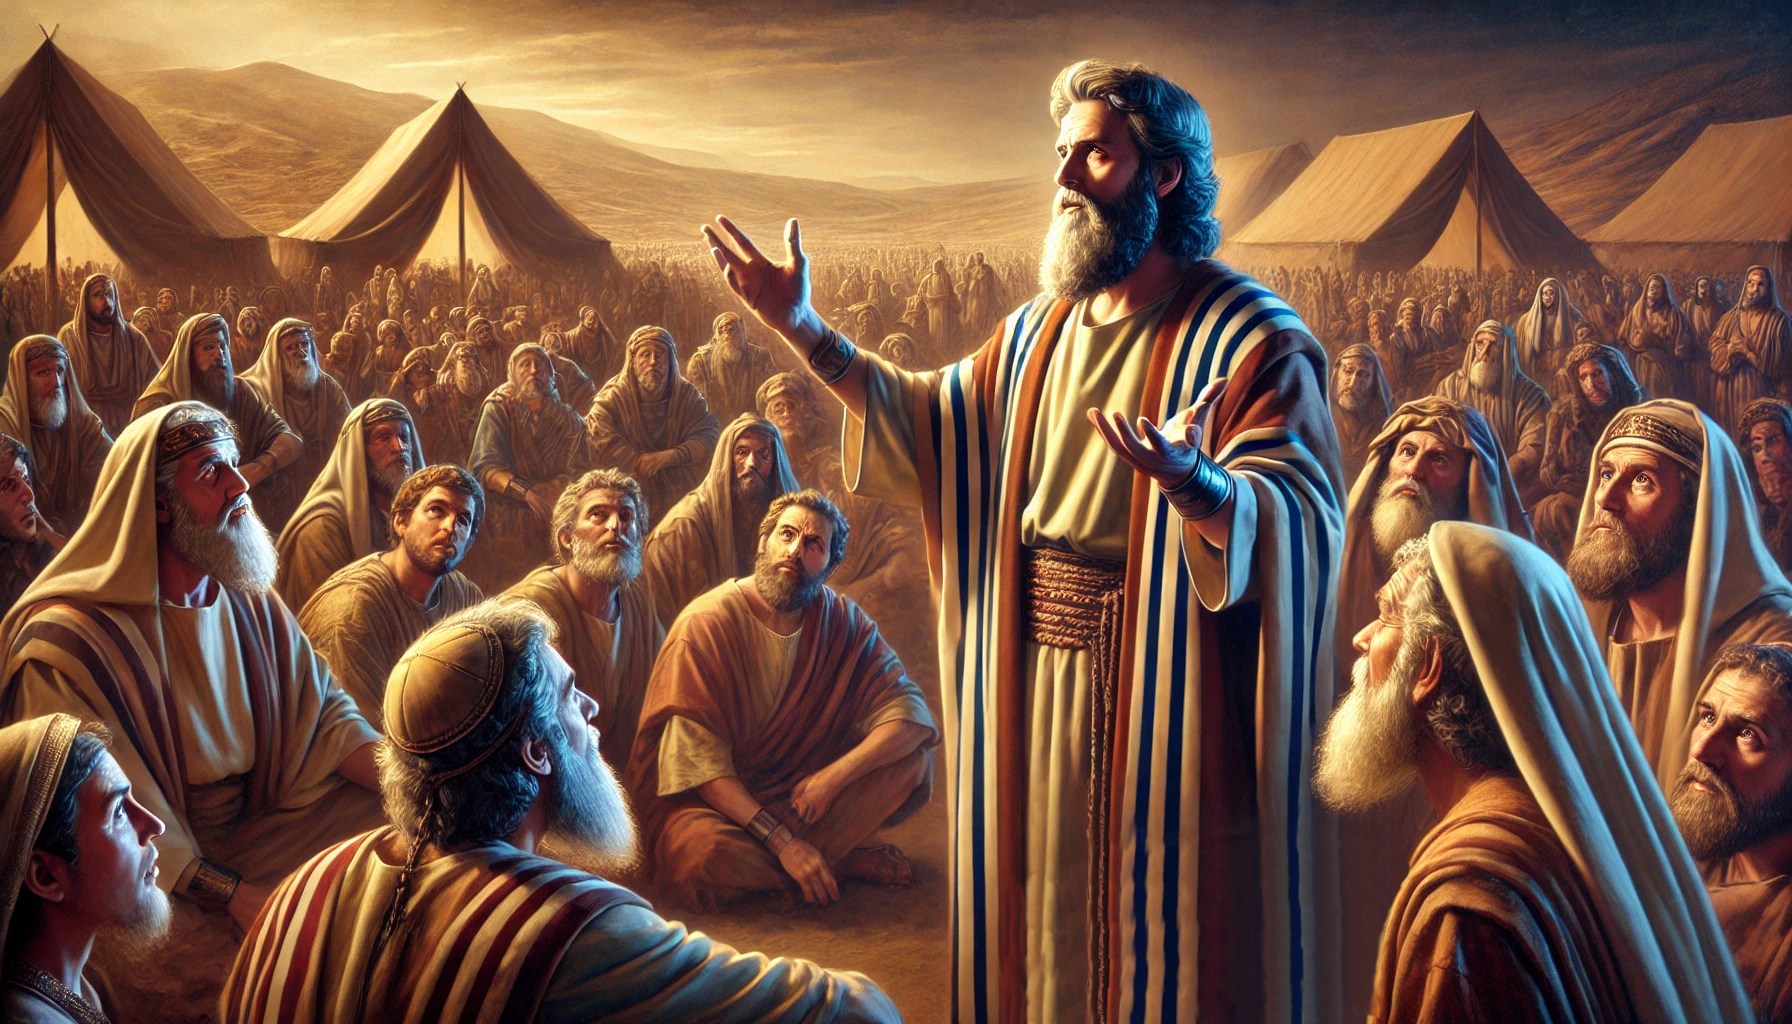
\includegraphics[width=0.7\linewidth]{graficas/levitico}\\
	Moisés ante el pueblo de Israel \\
\end{center}




\section*{Capítulo 1} 
Los holocaustos 

 
1:1 Llamó Jehová a Moisés, y habló con él desde el tabernáculo de reunión, diciendo:  
1:2 Habla a los hijos de Israel y diles: Cuando alguno de entre vosotros ofrece ofrenda a Jehová, de ganado vacuno u ovejuno haréis vuestra ofrenda.  
1:3 Si su ofrenda fuere holocausto vacuno, macho sin defecto lo ofrecerá; de su voluntad lo ofrecerá a la puerta del tabernáculo de reunión delante de Jehová.  
1:4 Y pondrá su mano sobre la cabeza del holocausto, y será aceptado para expiación suya.  
1:5 Entonces degollará el becerro en la presencia de Jehová; y los sacerdotes hijos de Aarón ofrecerán la sangre, y la rociarán alrededor sobre el altar, el cual está a la puerta del tabernáculo de reunión.  
1:6 Y desollará el holocausto, y lo dividirá en sus piezas.  
1:7 Y los hijos del sacerdote Aarón pondrán fuego sobre el altar, y compondrán la leña sobre el fuego.  
1:8 Luego los sacerdotes hijos de Aarón acomodarán las piezas, la cabeza y la grosura de los intestinos, sobre la leña que está sobre el fuego que habrá encima del altar;  
1:9 y lavará con agua los intestinos y las piernas, y el sacerdote hará arder todo sobre el altar; holocausto es, ofrenda encendida de olor grato para Jehová.  
1:10 Si su ofrenda para holocausto fuere del rebaño, de las ovejas o de las cabras, macho sin defecto lo ofrecerá.  
1:11 Y lo degollará al lado norte del altar delante de Jehová; y los sacerdotes hijos de Aarón rociarán su sangre sobre el altar alrededor.  
1:12 Lo dividirá en sus piezas, con su cabeza y la grosura de los intestinos; y el sacerdote las acomodará sobre la leña que está sobre el fuego que habrá encima del altar; 
1:13 y lavará las entrañas y las piernas con agua; y el sacerdote lo ofrecerá todo, y lo hará arder sobre el altar; holocausto es, ofrenda encendida de olor grato para Jehová.  
1:14 Si la ofrenda para Jehová fuere holocausto de aves, presentará su ofrenda de tórtolas, o de palominos.  
1:15 Y el sacerdote la ofrecerá sobre el altar, y le quitará la cabeza, y hará que arda en el altar; y su sangre será exprimida sobre la pared del altar.  
1:16 Y le quitará el buche y las plumas, lo cual echará junto al altar, hacia el oriente, en el lugar de las cenizas.  
1:17 Y la henderá por sus alas, pero no la dividirá en dos; y el sacerdote la hará arder sobre el altar, sobre la leña que estará en el fuego; holocausto es, ofrenda encendida de olor grato para Jehová.  
\section*{Capítulo 2}
Las ofrendas 

2:1 Cuando alguna persona ofreciere oblación a Jehová, su ofrenda será flor de harina, sobre la cual echará aceite, y pondrá sobre ella incienso,  
2:2 y la traerá a los sacerdotes, hijos de Aarón; y de ello tomará el sacerdote su puño lleno de la flor de harina y del aceite, con todo el incienso, y lo hará arder sobre el altar para memorial; ofrenda encendida es, de olor grato a Jehová.  
2:3 Y lo que resta de la ofrenda será de Aarón y de sus hijos; es cosa santísima de las ofrendas que se queman para Jehová.  
2:4 Cuando ofrecieres ofrenda cocida en horno, será de tortas de flor de harina sin levadura amasadas con aceite, y hojaldres sin levadura untadas con aceite.  
2:5 Mas si ofrecieres ofrenda de sartén, será de flor de harina sin levadura, amasada con aceite,  
2:6 la cual partirás en piezas, y echarás sobre ella aceite; es ofrenda.  
2:7 Si ofrecieres ofrenda cocida en cazuela, se hará de flor de harina con aceite.  
2:8 Y traerás a Jehová la ofrenda que se hará de estas cosas, y la presentarás al sacerdote, el cual la llevará al altar.  
2:9 Y tomará el sacerdote de aquella ofrenda lo que sea para su memorial, y lo hará arder sobre el altar; ofrenda encendida de olor grato a Jehová.  
2:10 Y lo que resta de la ofrenda será de Aarón y de sus hijos; es cosa santísima de las ofrendas que se queman para Jehová.  
2:11 Ninguna ofrenda que ofreciereis a Jehová será con levadura; porque de ninguna cosa leuda, ni de ninguna miel, se ha de quemar ofrenda para Jehová.  
2:12 Como ofrenda de primicias las ofreceréis a Jehová; mas no subirán sobre el altar en olor grato.  
2:13 Y sazonarás con sal toda ofrenda que presentes, y no harás que falte jamás de tu ofrenda la sal del pacto de tu Dios; en toda ofrenda tuya ofrecerás sal.  
2:14 Si ofrecieres a Jehová ofrenda de primicias, tostarás al fuego las espigas verdes, y el grano desmenuzado ofrecerás como ofrenda de tus primicias.  
2:15 Y pondrás sobre ella aceite, y pondrás sobre ella incienso; es ofrenda.  
2:16 Y el sacerdote hará arder el memorial de él, parte del grano desmenuzado y del aceite, con todo el incienso; es ofrenda encendida para Jehová.  
\section*{Capítulo 3}
Ofrendas de paz  

3:1 Si su ofrenda fuere sacrificio de paz, si hubiere de ofrecerla de ganado vacuno, sea macho o hembra, sin defecto la ofrecerá delante de Jehová. 
3:2 Pondrá su mano sobre la cabeza de su ofrenda, y la degollará a la puerta del tabernáculo de reunión; y los sacerdotes hijos de Aarón rociarán su sangre sobre el altar alrededor.  
3:3 Luego ofrecerá del sacrificio de paz, como ofrenda encendida a Jehová, la grosura que cubre los intestinos, y toda la grosura que está sobre las entrañas,  
3:4 y los dos riñones y la grosura que está sobre ellos, y sobre los ijares; y con los riñones quitará la grosura de los intestinos que está sobre el hígado.  
3:5 Y los hijos de Aarón harán arder esto en el altar, sobre el holocausto que estará sobre la leña que habrá encima del fuego; es ofrenda de olor grato para Jehová.  
3:6 Mas si de ovejas fuere su ofrenda para sacrificio de paz a Jehová, sea macho o hembra, la ofrecerá sin defecto.  
3:7 Si ofreciere cordero por su ofrenda, lo ofrecerá delante de Jehová.  
3:8 Pondrá su mano sobre la cabeza de su ofrenda, y después la degollará delante del tabernáculo de reunión; y los hijos de Aarón rociarán su sangre sobre el altar alrededor.  
3:9 Y del sacrificio de paz ofrecerá por ofrenda encendida a Jehová la grosura, la cola entera, la cual quitará a raíz del espinazo, la grosura que cubre todos los intestinos, y toda la que está sobre las entrañas.  
3:10 Asimismo los dos riñones y la grosura que está sobre ellos, y la que está sobre los ijares; y con los riñones quitará la grosura de sobre el hígado.  
3:11 Y el sacerdote hará arder esto sobre el altar; vianda es de ofrenda encendida para Jehová.  
3:12 Si fuere cabra su ofrenda, la ofrecerá delante de Jehová.  
3:13 Pondrá su mano sobre la cabeza de ella, y la degollará delante del tabernáculo de reunión; y los hijos de Aarón rociarán su sangre sobre el altar alrededor.  
3:14 Después ofrecerá de ella su ofrenda encendida a Jehová; la grosura que cubre los intestinos, y toda la grosura que está sobre las entrañas,  
3:15 los dos riñones, la grosura que está sobre ellos, y la que está sobre los ijares; y con los riñones quitará la grosura de sobre el hígado.  
3:16 Y el sacerdote hará arder esto sobre el altar; vianda es de ofrenda que se quema en olor grato a Jehová; toda la grosura es de Jehová.  
3:17 Estatuto perpetuo será por vuestras edades, dondequiera que habitéis, que ninguna grosura ni ninguna sangre comeréis.  
\section*{Capítulo 4 }
Ofrendas por el pecado  

4:1 Habló Jehová a Moisés, diciendo:  
4:2 Habla a los hijos de Israel y diles: Cuando alguna persona pecare por yerro en alguno de los mandamientos de Jehová sobre cosas que no se han de hacer, e hiciere alguna de ellas;  
4:3 si el sacerdote ungido pecare según el pecado del pueblo, ofrecerá a Jehová, por su pecado que habrá cometido, un becerro sin defecto para expiación.  
4:4 Traerá el becerro a la puerta del tabernáculo de reunión delante de Jehová, y pondrá su mano sobre la cabeza del becerro, y lo degollará delante de Jehová.  
4:5 Y el sacerdote ungido tomará de la sangre del becerro, y la traerá al tabernáculo de reunión;  
4:6 y mojará el sacerdote su dedo en la sangre, y rociará de aquella sangre siete veces delante de Jehová, hacia el velo del santuario.  
4:7 Y el sacerdote pondrá de esa sangre sobre los cuernos del altar del incienso aromático, que está en el tabernáculo de reunión delante de Jehová; y echará el resto de la sangre del becerro al pie del altar del holocausto, que está a la puerta del tabernáculo de reunión.  
4:8 Y tomará del becerro para la expiación toda su grosura, la que cubre los intestinos, y la que está sobre las entrañas,  
4:9 los dos riñones, la grosura que está sobre ellos, y la que está sobre los ijares; y con los riñones quitará la grosura de sobre el hígado,  
4:10 de la manera que se quita del buey del sacrificio de paz; y el sacerdote la hará arder sobre el altar del holocausto.  
4:11 Y la piel del becerro, y toda su carne, con su cabeza, sus piernas, sus intestinos y su estiércol,  
4:12 en fin, todo el becerro sacará fuera del campamento a un lugar limpio, donde se echan las cenizas, y lo quemará al fuego sobre la leña; en donde se echan las cenizas será quemado.  
4:13 Si toda la congregación de Israel hubiere errado, y el yerro estuviere oculto a los ojos del pueblo, y hubieren hecho algo contra alguno de los mandamientos de Jehová en cosas que no se han de hacer, y fueren culpables;  
4:14 luego que llegue a ser conocido el pecado que cometieren, la congregación ofrecerá un becerro por expiación, y lo traerán delante del tabernáculo de reunión.  
4:15 Y los ancianos de la congregación pondrán sus manos sobre la cabeza del becerro delante de Jehová, y en presencia de Jehová degollarán aquel becerro.  
4:16 Y el sacerdote ungido meterá de la sangre del becerro en el tabernáculo de reunión,  
4:17 y mojará el sacerdote su dedo en la misma sangre, y rociará siete veces delante de Jehová hacia el velo.  
4:18 Y de aquella sangre pondrá sobre los cuernos del altar que está delante de Jehová en el tabernáculo de reunión, y derramará el resto de la sangre al pie del altar del holocausto, que está a la puerta del tabernáculo de reunión.  
4:19 Y le quitará toda la grosura y la hará arder sobre el altar.  
4:20 Y hará de aquel becerro como hizo con el becerro de la expiación; lo mismo hará de él; así hará el sacerdote expiación por ellos, y obtendrán perdón.  
4:21 Y sacará el becerro fuera del campamento, y lo quemará como quemó el primer becerro; expiación es por la congregación.  
4:22 Cuando pecare un jefe, e hiciere por yerro algo contra alguno de todos los mandamientos de Jehová su Dios sobre cosas que no se han de hacer, y pecare;  
4:23 luego que conociere su pecado que cometió, presentará por su ofrenda un macho cabrío sin defecto.  
4:24 Y pondrá su mano sobre la cabeza del macho cabrío, y lo degollará en el lugar donde se degüella el holocausto, delante de Jehová; es expiación.  
4:25 Y con su dedo el sacerdote tomará de la sangre de la expiación, y la pondrá sobre los cuernos del altar del holocausto, y derramará el resto de la sangre al pie del altar del holocausto,  
4:26 y quemará toda su grosura sobre el altar, como la grosura del sacrificio de paz; así el sacerdote hará por él la expiación de su pecado, y tendrá perdón.  
4:27 Si alguna persona del pueblo pecare por yerro, haciendo algo contra alguno de los mandamientos de Jehová en cosas que no se han de hacer, y delinquiere;  
4:28 luego que conociere su pecado que cometió, traerá por su ofrenda una cabra, una cabra sin defecto, por su pecado que cometió.  
4:29 Y pondrá su mano sobre la cabeza de la ofrenda de la expiación, y la degollará en el lugar del holocausto.  
4:30 Luego con su dedo el sacerdote tomará de la sangre, y la pondrá sobre los cuernos del altar del holocausto, y derramará el resto de la sangre al pie del altar.  
4:31 Y le quitará toda su grosura, de la manera que fue quitada la grosura del sacrificio de paz; y el sacerdote la hará arder sobre el altar en olor grato a Jehová; así hará el sacerdote expiación por él, y será perdonado. 
4:32 Y si por su ofrenda por el pecado trajere cordero, hembra sin defecto traerá.  
4:33 Y pondrá su mano sobre la cabeza de la ofrenda de expiación, y la degollará por expiación en el lugar donde se degüella el holocausto.  
4:34 Después con su dedo el sacerdote tomará de la sangre de la expiación, y la pondrá sobre los cuernos del altar del holocausto, y derramará el resto de la sangre al pie del altar.  
4:35 Y le quitará toda su grosura, como fue quitada la grosura del sacrificio de paz, y el sacerdote la hará arder en el altar sobre la ofrenda encendida a Jehová; y le hará el sacerdote expiación de su pecado que habrá cometido, y será perdonado.  
\section*{Capítulo 5 }

5:1 Si alguno pecare por haber sido llamado a testificar, y fuere testigo que vio, o supo, y no lo denunciare, él llevará su pecado.  
5:2 Asimismo la persona que hubiere tocado cualquiera cosa inmunda, sea cadáver de bestia inmunda, o cadáver de animal inmundo, o cadáver de reptil inmundo, bien que no lo supiere, será inmunda y habrá delinquido.  
5:3 O si tocare inmundicia de hombre, cualquiera inmundicia suya con que fuere inmundo, y no lo echare de ver, si después llegare a saberlo, será culpable.  
5:4 O si alguno jurare a la ligera con sus labios hacer mal o hacer bien, en cualquiera cosa que el hombre profiere con juramento, y él no lo entendiere; si después lo entiende, será culpable por cualquiera de estas cosas.  
5:5 Cuando pecare en alguna de estas cosas, confesará aquello en que pecó,  
5:6 y para su expiación traerá a Jehová por su pecado que cometió, una hembra de los rebaños, una cordera o una cabra como ofrenda de expiación; y el sacerdote le hará expiación por su pecado.  
5:7 Y si no tuviere lo suficiente para un cordero, traerá a Jehová en expiación por su pecado que cometió, dos tórtolas o dos palominos, el uno para expiación, y el otro para holocausto.  
5:8 Y los traerá al sacerdote, el cual ofrecerá primero el que es para expiación; y le arrancará de su cuello la cabeza, mas no la separará por completo.  
5:9 Y rociará de la sangre de la expiación sobre la pared del altar; y lo que sobrare de la sangre lo exprimirá al pie del altar; es expiación.  
5:10 Y del otro hará holocausto conforme al rito; así el sacerdote hará expiación por el pecado de aquel que lo cometió, y será perdonado. 
5:11 Mas si no tuviere lo suficiente para dos tórtolas, o dos palominos, el que pecó traerá como ofrenda la décima parte de un efa  de flor de harina para expiación. No pondrá sobre ella aceite, ni sobre ella pondrá incienso, porque es expiación.  
5:12 La traerá, pues, al sacerdote, y el sacerdote tomará de ella su puño lleno, para memoria de él, y la hará arder en el altar sobre las ofrendas encendidas a Jehová; es expiación.  
5:13 Y hará el sacerdote expiación por él en cuanto al pecado que cometió en alguna de estas cosas, y será perdonado; y el sobrante será del sacerdote, como la ofrenda de vianda.  
Ofrendas expiatorias  
5:14 Habló más Jehová a Moisés, diciendo:  
5:15 Cuando alguna persona cometiere falta, y pecare por yerro en las cosas santas de Jehová, traerá por su culpa a Jehová un carnero sin defecto de los rebaños, conforme a tu estimación en siclos de plata  del siclo del santuario, en ofrenda por el pecado.  
5:16 Y pagará lo que hubiere defraudado de las cosas santas, y añadirá a ello la quinta parte, y lo dará al sacerdote; y el sacerdote hará expiación por él con el carnero del sacrificio por el pecado, y será perdonado.  
5:17 Finalmente, si una persona pecare, o hiciere alguna de todas aquellas cosas que por mandamiento de Jehová no se han de hacer, aun sin hacerlo a sabiendas, es culpable, y llevará su pecado.  
5:18 Traerá, pues, al sacerdote para expiación, según tú lo estimes, un carnero sin defecto de los rebaños; y el sacerdote le hará expiación por el yerro que cometió por ignorancia, y será perdonado.  
5:19 Es infracción, y ciertamente delinquió contra Jehová.  
\section*{Capítulo 6 }

6:1 Habló Jehová a Moisés, diciendo:  
6:2 Cuando una persona pecare e hiciere prevaricación contra Jehová, y negare a su prójimo lo encomendado o dejado en su mano, o bien robare o calumniare a su prójimo,  
6:3 o habiendo hallado lo perdido después lo negare, y jurare en falso; en alguna de todas aquellas cosas en que suele pecar el hombre,  
6:4 entonces, habiendo pecado y ofendido, restituirá aquello que robó, o el daño de la calumnia, o el depósito que se le encomendó, o lo perdido que halló,  
6:5 o todo aquello sobre que hubiere jurado falsamente; lo restituirá por entero a aquel a quien pertenece, y añadirá a ello la quinta parte, en el día de su expiación.  
6:6 Y para expiación de su culpa traerá a Jehová un carnero sin defecto de los rebaños, conforme a tu estimación, y lo dará al sacerdote para la expiación.  
6:7 Y el sacerdote hará expiación por él delante de Jehová, y obtendrá perdón de cualquiera de todas las cosas en que suele ofender.  
Leyes de los sacrificios  
6:8 Habló aún Jehová a Moisés, diciendo:  
6:9 Manda a Aarón y a sus hijos, y diles: Esta es la ley del holocausto: el holocausto estará sobre el fuego encendido sobre el altar toda la noche, hasta la mañana; el fuego del altar arderá en él.  
6:10 Y el sacerdote se pondrá su vestidura de lino, y vestirá calzoncillos de lino sobre su cuerpo; y cuando el fuego hubiere consumido el holocausto, apartará él las cenizas de sobre el altar, y las pondrá junto al altar.  
6:11 Después se quitará sus vestiduras y se pondrá otras ropas, y sacará las cenizas fuera del campamento a un lugar limpio.  
6:12 Y el fuego encendido sobre el altar no se apagará, sino que el sacerdote pondrá en él leña cada mañana, y acomodará el holocausto sobre él, y quemará sobre él las grosuras de los sacrificios de paz.  
6:13 El fuego arderá continuamente en el altar; no se apagará.  
6:14 Esta es la ley de la ofrenda: La ofrecerán los hijos de Aarón delante de Jehová ante el altar.  
6:15 Y tomará de ella un puñado de la flor de harina de la ofrenda, y de su aceite, y todo el incienso que está sobre la ofrenda, y lo hará arder sobre el altar por memorial en olor grato a Jehová.  
6:16 Y el sobrante de ella lo comerán Aarón y sus hijos; sin levadura se comerá en lugar santo; en el atrio del tabernáculo de reunión lo comerán.  
6:17 No se cocerá con levadura; la he dado a ellos por su porción de mis ofrendas encendidas; es cosa santísima, como el sacrificio por el pecado, y como el sacrificio por la culpa.  
6:18 Todos los varones de los hijos de Aarón comerán de ella. Estatuto perpetuo será para vuestras generaciones tocante a las ofrendas encendidas para Jehová; toda cosa que tocare en ellas será santificada.  
6:19 Habló también Jehová a Moisés, diciendo:  
6:20 Esta es la ofrenda de Aarón y de sus hijos, que ofrecerán a Jehová el día que fueren ungidos: la décima parte de un efa  de flor de harina, ofrenda perpetua, la mitad a la mañana y la mitad a la tarde.  
6:21 En sartén se preparará con aceite; frita la traerás, y los pedazos cocidos de la ofrenda ofrecerás en olor grato a Jehová.  
6:22 Y el sacerdote que en lugar de Aarón fuere ungido de entre sus hijos, hará igual ofrenda. Es estatuto perpetuo de Jehová; toda ella será quemada.  
6:23 Toda ofrenda de sacerdote será enteramente quemada; no se comerá.  
6:24 Y habló Jehová a Moisés, diciendo:  
6:25 Habla a Aarón y a sus hijos, y diles: Esta es la ley del sacrificio expiatorio: en el lugar donde se degüella el holocausto, será degollada la ofrenda por el pecado delante de Jehová; es cosa santísima.  
6:26 El sacerdote que la ofreciere por el pecado, la comerá; en lugar santo será comida, en el atrio del tabernáculo de reunión.  
6:27 Todo lo que tocare su carne, será santificado; y si salpicare su sangre sobre el vestido, lavarás aquello sobre que cayere, en lugar santo.  
6:28 Y la vasija de barro en que fuere cocida, será quebrada; y si fuere cocida en vasija de bronce, será fregada y lavada con agua. 
6:29 Todo varón de entre los sacerdotes la comerá; es cosa santísima.  
6:30 Mas no se comerá ninguna ofrenda de cuya sangre se metiere en el tabernáculo de reunión para hacer expiación en el santuario; al fuego será quemada.  
\section*{Capítulo 7 }

7:1 Asimismo esta es la ley del sacrificio por la culpa; es cosa muy santa.  
7:2 En el lugar donde degüellan el holocausto, degollarán la víctima por la culpa; y rociará su sangre alrededor sobre el altar.  
7:3 Y de ella ofrecerá toda su grosura, la cola, y la grosura que cubre los intestinos,  
7:4 los dos riñones, la grosura que está sobre ellos, y la que está sobre los ijares; y con los riñones quitará la grosura de sobre el hígado.  
7:5 Y el sacerdote lo hará arder sobre el altar, ofrenda encendida a Jehová; es expiación de la culpa.  
7:6 Todo varón de entre los sacerdotes la comerá; será comida en lugar santo; es cosa muy santa.  
7:7 Como el sacrificio por el pecado, así es el sacrificio por la culpa; una misma ley tendrán; será del sacerdote que hiciere la expiación con ella.  
7:8 Y el sacerdote que ofreciere holocausto de alguno, la piel del holocausto que ofreciere será para él.  
7:9 Asimismo toda ofrenda que se cociere en horno, y todo lo que fuere preparado en sartén o en cazuela, será del sacerdote que lo ofreciere.  
7:10 Y toda ofrenda amasada con aceite, o seca, será de todos los hijos de Aarón, tanto de uno como de otro.  
7:11 Y esta es la ley del sacrificio de paz que se ofrecerá a Jehová:  
7:12 Si se ofreciere en acción de gracias, ofrecerá por sacrificio de acción de gracias tortas sin levadura amasadas con aceite, y hojaldres sin levadura untadas con aceite, y flor de harina frita en tortas amasadas con aceite.  
7:13 Con tortas de pan leudo presentará su ofrenda en el sacrificio de acciones de gracias de paz.  
7:14 Y de toda la ofrenda presentará una parte por ofrenda elevada a Jehová, y será del sacerdote que rociare la sangre de los sacrificios de paz.  
7:15 Y la carne del sacrificio de paz en acción de gracias se comerá en el día que fuere ofrecida; no dejarán de ella nada para otro día.  
7:16 Mas si el sacrificio de su ofrenda fuere voto, o voluntario, será comido en el día que ofreciere su sacrificio, y lo que de él quedare, lo comerán al día siguiente;  
7:17 y lo que quedare de la carne del sacrificio hasta el tercer día, será quemado en el fuego.  
7:18 Si se comiere de la carne del sacrificio de paz al tercer día, el que lo ofreciere no será acepto, ni le será contado; abominación será, y la persona que de él comiere llevará su pecado.  
7:19 Y la carne que tocare alguna cosa inmunda, no se comerá; al fuego será quemada. Toda persona limpia podrá comer la carne;  
7:20 pero la persona que comiere la carne del sacrificio de paz, el cual es de Jehová, estando inmunda, aquella persona será cortada de entre su pueblo.  
7:21 Además, la persona que tocare alguna cosa inmunda, inmundicia de hombre, o animal inmundo, o cualquier abominación inmunda, y comiere la carne del sacrificio de paz, el cual es de Jehová, aquella persona será cortada de entre su pueblo.  
7:22 Habló más Jehová a Moisés, diciendo:  
7:23 Habla a los hijos de Israel, diciendo: Ninguna grosura de buey ni de cordero ni de cabra comeréis.  
7:24 La grosura de animal muerto, y la grosura del que fue despedazado por fieras, se dispondrá para cualquier otro uso, mas no la comeréis.  
7:25 Porque cualquiera que comiere grosura de animal, del cual se ofrece a Jehová ofrenda encendida, la persona que lo comiere será cortada de entre su pueblo.  
7:26 Además, ninguna sangre comeréis en ningún lugar en donde habitéis, ni de aves ni de bestias. 
7:27 Cualquiera persona que comiere de alguna sangre, la tal persona será cortada de entre su pueblo.  
7:28 Habló más Jehová a Moisés, diciendo:  
7:29 Habla a los hijos de Israel y diles: El que ofreciere sacrificio de paz a Jehová, traerá su ofrenda del sacrificio de paz ante Jehová.  
7:30 Sus manos traerán las ofrendas que se han de quemar ante Jehová; traerá la grosura con el pecho; el pecho para que sea mecido como sacrificio mecido delante de Jehová.  
7:31 Y la grosura la hará arder el sacerdote en el altar, mas el pecho será de Aarón y de sus hijos.  
7:32 Y daréis al sacerdote para ser elevada en ofrenda, la espaldilla derecha de vuestros sacrificios de paz. 
7:33 El que de los hijos de Aarón ofreciere la sangre de los sacrificios de paz, y la grosura, recibirá la espaldilla derecha como porción suya.  
7:34 Porque he tomado de los sacrificios de paz de los hijos de Israel el pecho que se mece y la espaldilla elevada en ofrenda, y lo he dado a Aarón el sacerdote y a sus hijos, como estatuto perpetuo para los hijos de Israel.  
7:35 Esta es la porción de Aarón y la porción de sus hijos, de las ofrendas encendidas a Jehová, desde el día que él los consagró para ser sacerdotes de Jehová,  
7:36 la cual mandó Jehová que les diesen, desde el día que él los ungió de entre los hijos de Israel, como estatuto perpetuo en sus generaciones.  
7:37 Esta es la ley del holocausto, de la ofrenda, del sacrificio por el pecado, del sacrificio por la culpa, de las consagraciones y del sacrificio de paz,  
7:38 la cual mandó Jehová a Moisés en el monte de Sinaí, el día que mandó a los hijos de Israel que ofreciesen sus ofrendas a Jehová, en el desierto de Sinaí. 
\section*{Capítulo 8 }
Consagración de Aarón y de sus hijos   

8:1 Habló Jehová a Moisés, diciendo:  
8:2 Toma a Aarón y a sus hijos con él, y las vestiduras, el aceite de la unción, el becerro de la expiación, los dos carneros, y el canastillo de los panes sin levadura;  
8:3 y reúne toda la congregación a la puerta del tabernáculo de reunión.  
8:4 Hizo, pues, Moisés como Jehová le mandó, y se reunió la congregación a la puerta del tabernáculo de reunión.  
8:5 Y dijo Moisés a la congregación: Esto es lo que Jehová ha mandado hacer.  
8:6 Entonces Moisés hizo acercarse a Aarón y a sus hijos, y los lavó con agua.  
8:7 Y puso sobre él la túnica, y le ciñó con el cinto; le vistió después el manto, y puso sobre él el efod, y lo ciñó con el cinto del efod, y lo ajustó con él.  
8:8 Luego le puso encima el pectoral, y puso dentro del mismo los Urim y Tumim.  
8:9 Después puso la mitra sobre su cabeza, y sobre la mitra, en frente, puso la lámina de oro, la diadema santa, como Jehová había mandado a Moisés.  
8:10 Y tomó Moisés el aceite de la unción y ungió el tabernáculo y todas las cosas que estaban en él, y las santificó.  
8:11 Y roció de él sobre el altar siete veces, y ungió el altar y todos sus utensilios, y la fuente y su base, para santificarlos.  
8:12 Y derramó del aceite de la unción sobre la cabeza de Aarón, y lo ungió para santificarlo.  
8:13 Después Moisés hizo acercarse los hijos de Aarón, y les vistió las túnicas, les ciñó con cintos, y les ajustó las tiaras, como Jehová lo había mandado a Moisés.  
8:14 Luego hizo traer el becerro de la expiación, y Aarón y sus hijos pusieron sus manos sobre la cabeza del becerro de la expiación,  
8:15 y lo degolló; y Moisés tomó la sangre, y puso con su dedo sobre los cuernos del altar alrededor, y purificó el altar; y echó la demás sangre al pie del altar, y lo santificó para reconciliar sobre él.  
8:16 Después tomó toda la grosura que estaba sobre los intestinos, y la grosura del hígado, y los dos riñones, y la grosura de ellos, y lo hizo arder Moisés sobre el altar.  
8:17 Mas el becerro, su piel, su carne y su estiércol, lo quemó al fuego fuera del campamento, como Jehová lo había mandado a Moisés.  
8:18 Después hizo que trajeran el carnero del holocausto, y Aarón y sus hijos pusieron sus manos sobre la cabeza del carnero;  
8:19 y lo degolló; y roció Moisés la sangre sobre el altar alrededor,  
8:20 y cortó el carnero en trozos; y Moisés hizo arder la cabeza, y los trozos, y la grosura.  
8:21 Lavó luego con agua los intestinos y las piernas, y quemó Moisés todo el carnero sobre el altar; holocausto de olor grato, ofrenda encendida para Jehová, como Jehová lo había mandado a Moisés.  
8:22 Después hizo que trajeran el otro carnero, el carnero de las consagraciones, y Aarón y sus hijos pusieron sus manos sobre la cabeza del carnero.  
8:23 Y lo degolló; y tomó Moisés de la sangre, y la puso sobre el lóbulo de la oreja derecha de Aarón, sobre el dedo pulgar de su mano derecha, y sobre el dedo pulgar de su pie derecho.  
8:24 Hizo acercarse luego los hijos de Aarón, y puso Moisés de la sangre sobre el lóbulo de sus orejas derechas, sobre los pulgares de sus manos derechas, y sobre los pulgares de sus pies derechos; y roció Moisés la sangre sobre el altar alrededor.  
8:25 Después tomó la grosura, la cola, toda la grosura que estaba sobre los intestinos, la grosura del hígado, los dos riñones y la grosura de ellos, y la espaldilla derecha.  
8:26 Y del canastillo de los panes sin levadura, que estaba delante de Jehová, tomó una torta sin levadura, y una torta de pan de aceite, y una hojaldre, y lo puso con la grosura y con la espaldilla derecha.  
8:27 Y lo puso todo en las manos de Aarón, y en las manos de sus hijos, e hizo mecerlo como ofrenda mecida delante de Jehová.  
8:28 Después tomó aquellas cosas Moisés de las manos de ellos, y las hizo arder en el altar sobre el holocausto; eran las consagraciones en olor grato, ofrenda encendida a Jehová.  
8:29 Y tomó Moisés el pecho, y lo meció, ofrenda mecida delante de Jehová; del carnero de las consagraciones aquella fue la parte de Moisés, como Jehová lo había mandado a Moisés.  
8:30 Luego tomó Moisés del aceite de la unción, y de la sangre que estaba sobre el altar, y roció sobre Aarón, y sobre sus vestiduras, sobre sus hijos, y sobre las vestiduras de sus hijos con él; y santificó a Aarón y sus vestiduras, y a sus hijos y las vestiduras de sus hijos con él.  
8:31 Y dijo Moisés a Aarón y a sus hijos: Hervid la carne a la puerta del tabernáculo de reunión; y comedla allí con el pan que está en el canastillo de las consagraciones, según yo he mandado, diciendo: Aarón y sus hijos la comerán.  
8:32 Y lo que sobre de la carne y del pan, lo quemaréis al fuego.  
8:33 De la puerta del tabernáculo de reunión no saldréis en siete días, hasta el día que se cumplan los días de vuestras consagraciones; porque por siete días seréis consagrados.  
8:34 De la manera que hoy se ha hecho, mandó hacer Jehová para expiaros.  
8:35 A la puerta, pues, del tabernáculo de reunión estaréis día y noche por siete días, y guardaréis la ordenanza delante de Jehová, para que no muráis; porque así me ha sido mandado.  
8:36 Y Aarón y sus hijos hicieron todas las cosas que mandó Jehová por medio de Moisés.  
\section*{Capítulo 9 }
Los sacrificios de Aarón  

9:1 En el día octavo, Moisés llamó a Aarón y a sus hijos, y a los ancianos de Israel;  
9:2 y dijo a Aarón: Toma de la vacada un becerro para expiación, y un carnero para holocausto, sin defecto, y ofrécelos delante de Jehová.  
9:3 Y a los hijos de Israel hablarás diciendo: Tomad un macho cabrío para expiación, y un becerro y un cordero de un año, sin defecto, para holocausto.  
9:4 Asimismo un buey y un carnero para sacrificio de paz, que inmoléis delante de Jehová, y una ofrenda amasada con aceite; porque Jehová se aparecerá hoy a vosotros.  
9:5 Y llevaron lo que mandó Moisés delante del tabernáculo de reunión, y vino toda la congregación y se puso delante de Jehová.  
9:6 Entonces Moisés dijo: Esto es lo que mandó Jehová; hacedlo, y la gloria de Jehová se os aparecerá.  
9:7 Y dijo Moisés a Aarón: Acércate al altar, y haz tu expiación y tu holocausto, y haz la reconciliación por ti y por el pueblo; haz también la ofrenda del pueblo, y haz la reconciliación por ellos, como ha mandado Jehová.  
9:8 Entonces se acercó Aarón al altar y degolló el becerro de la expiación que era por él.  
9:9 Y los hijos de Aarón le trajeron la sangre; y él mojó su dedo en la sangre, y puso de ella sobre los cuernos del altar, y derramó el resto de la sangre al pie del altar.  
9:10 E hizo arder sobre el altar la grosura con los riñones y la grosura del hígado de la expiación, como Jehová lo había mandado a Moisés.  
9:11 Mas la carne y la piel las quemó al fuego fuera del campamento.  
9:12 Degolló asimismo el holocausto, y los hijos de Aarón le presentaron la sangre, la cual roció él alrededor sobre el altar.  
9:13 Después le presentaron el holocausto pieza por pieza, y la cabeza; y lo hizo quemar sobre el altar.  
9:14 Luego lavó los intestinos y las piernas, y los quemó sobre el holocausto en el altar.  
9:15 Ofreció también la ofrenda del pueblo, y tomó el macho cabrío que era para la expiación del pueblo, y lo degolló, y lo ofreció por el pecado como el primero.  
9:16 Y ofreció el holocausto, e hizo según el rito.  
9:17 Ofreció asimismo la ofrenda, y llenó de ella su mano, y la hizo quemar sobre el altar, además del holocausto de la mañana.  
9:18 Degolló también el buey y el carnero en sacrificio de paz, que era del pueblo; y los hijos de Aarón le presentaron la sangre, la cual roció él sobre el altar alrededor;  
9:19 y las grosuras del buey y del carnero, la cola, la grosura que cubre los intestinos, los riñones, y la grosura del hígado;  
9:20 y pusieron las grosuras sobre los pechos, y él las quemó sobre el altar.  
9:21 Pero los pechos, con la espaldilla derecha, los meció Aarón como ofrenda mecida delante de Jehová, como Jehová lo había mandado a Moisés.  
9:22 Después alzó Aarón sus manos hacia el pueblo y lo bendijo; y después de hacer la expiación, el holocausto y el sacrificio de paz, descendió.  
9:23 Y entraron Moisés y Aarón en el tabernáculo de reunión, y salieron y bendijeron al pueblo; y la gloria de Jehová se apareció a todo el pueblo.  
9:24 Y salió fuego de delante de Jehová, y consumió el holocausto con las grosuras sobre el altar; y viéndolo todo el pueblo, alabaron, y se postraron sobre sus rostros.  
\section*{Capítulo 10}
El pecado de Nadab y Abiú  

10:1 Nadab y Abiú, hijos de Aarón, tomaron cada uno su incensario, y pusieron en ellos fuego, sobre el cual pusieron incienso, y ofrecieron delante de Jehová fuego extraño, que él nunca les mandó.  
10:2 Y salió fuego de delante de Jehová y los quemó, y murieron delante de Jehová.  
10:3 Entonces dijo Moisés a Aarón: Esto es lo que habló Jehová, diciendo: En los que a mí se acercan me santificaré, y en presencia de todo el pueblo seré glorificado. Y Aarón calló.  
10:4 Y llamó Moisés a Misael y a Elzafán, hijos de Uziel tío de Aarón, y les dijo: Acercaos y sacad a vuestros hermanos de delante del santuario, fuera del campamento.  
10:5 Y ellos se acercaron y los sacaron con sus túnicas fuera del campamento, como dijo Moisés.  
10:6 Entonces Moisés dijo a Aarón, y a Eleazar e Itamar sus hijos: No descubráis vuestras cabezas, ni rasguéis vuestros vestidos en señal de duelo, para que no muráis, ni se levante la ira sobre toda la congregación; pero vuestros hermanos, toda la casa de Israel, sí lamentarán por el incendio que Jehová ha hecho.  
10:7 Ni saldréis de la puerta del tabernáculo de reunión, porque moriréis; por cuanto el aceite de la unción de Jehová está sobre vosotros. Y ellos hicieron conforme al dicho de Moisés.  
10:8 Y Jehová habló a Aarón, diciendo:  
10:9 Tú, y tus hijos contigo, no beberéis vino ni sidra cuando entréis en el tabernáculo de reunión, para que no muráis; estatuto perpetuo será para vuestras generaciones,  
10:10 para poder discernir entre lo santo y lo profano, y entre lo inmundo y lo limpio,  
10:11 y para enseñar a los hijos de Israel todos los estatutos que Jehová les ha dicho por medio de Moisés.  
10:12 Y Moisés dijo a Aarón, y a Eleazar y a Itamar sus hijos que habían quedado: Tomad la ofrenda que queda de las ofrendas encendidas a Jehová, y comedla sin levadura junto al altar, porque es cosa muy santa.  
10:13 La comeréis, pues, en lugar santo; porque esto es para ti y para tus hijos, de las ofrendas encendidas a Jehová, pues que así me ha sido mandado. 
10:14 Comeréis asimismo en lugar limpio, tú y tus hijos y tus hijas contigo, el pecho mecido y la espaldilla elevada, porque por derecho son tuyos y de tus hijos, dados de los sacrificios de paz de los hijos de Israel.  
10:15 Con las ofrendas de las grosuras que se han de quemar, traerán la espaldilla que se ha de elevar y el pecho que será mecido como ofrenda mecida delante de Jehová; y será por derecho perpetuo tuyo y de tus hijos, como Jehová lo ha mandado.  
10:16 Y Moisés preguntó por el macho cabrío de la expiación, y se halló que había sido quemado; y se enojó contra Eleazar e Itamar, los hijos que habían quedado de Aarón, diciendo:  
10:17 ¿Por qué no comisteis la expiación en lugar santo? Pues es muy santa, y la dio él a vosotros para llevar la iniquidad de la congregación, para que sean reconciliados delante de Jehová.  
10:18 Ved que la sangre no fue llevada dentro del santuario; y vosotros debíais comer la ofrenda en el lugar santo, como yo mandé.  
10:19 Y respondió Aarón a Moisés: He aquí hoy han ofrecido su expiación y su holocausto delante de Jehová; pero a mí me han sucedido estas cosas, y si hubiera yo comido hoy del sacrificio de expiación, ¿sería esto grato a Jehová?  
10:20 Y cuando Moisés oyó esto, se dio por satisfecho.  
\section*{Capítulo 11}
Animales limpios e inmundos  

11:1 Habló Jehová a Moisés y a Aarón, diciéndoles:  
11:2 Hablad a los hijos de Israel y decidles: Estos son los animales que comeréis de entre todos los animales que hay sobre la tierra.  
11:3 De entre los animales, todo el que tiene pezuña hendida y que rumia, éste comeréis.  
11:4 Pero de los que rumian o que tienen pezuña, no comeréis éstos: el camello, porque rumia pero no tiene pezuña hendida, lo tendréis por inmundo.  
11:5 También el conejo, porque rumia, pero no tiene pezuña, lo tendréis por inmundo.  
11:6 Asimismo la liebre, porque rumia, pero no tiene pezuña, la tendréis por inmunda.  
11:7 También el cerdo, porque tiene pezuñas, y es de pezuñas hendidas, pero no rumia, lo tendréis por inmundo.  
11:8 De la carne de ellos no comeréis, ni tocaréis su cuerpo muerto; los tendréis por inmundos.  
11:9 Esto comeréis de todos los animales que viven en las aguas: todos los que tienen aletas y escamas en las aguas del mar, y en los ríos, estos comeréis.  
11:10 Pero todos los que no tienen aletas ni escamas en el mar y en los ríos, así de todo lo que se mueve como de toda cosa viviente que está en las aguas, los tendréis en abominación. 
11:11 Os serán, pues, abominación; de su carne no comeréis, y abominaréis sus cuerpos muertos.  
11:12 Todo lo que no tuviere aletas y escamas en las aguas, lo tendréis en abominación.  
11:13 Y de las aves, éstas tendréis en abominación; no se comerán, serán abominación: el águila, el quebrantahuesos, el azor,  
11:14 el gallinazo, el milano según su especie;  
11:15 todo cuervo según su especie;  
11:16 el avestruz, la lechuza, la gaviota, el gavilán según su especie;  
11:17 el buho, el somormujo, el ibis,  
11:18 el calamón, el pelícano, el buitre,  
11:19 la cigüeña, la garza según su especie, la abubilla y el murciélago.  
11:20 Todo insecto alado que anduviere sobre cuatro patas, tendréis en abominación.  
11:21 Pero esto comeréis de todo insecto alado que anda sobre cuatro patas, que tuviere piernas además de sus patas para saltar con ellas sobre la tierra;  
11:22 estos comeréis de ellos: la langosta según su especie, el langostín según su especie, el argol según su especie, y el hagab según su especie.  
11:23 Todo insecto alado que tenga cuatro patas, tendréis en abominación.  
11:24 Y por estas cosas seréis inmundos; cualquiera que tocare sus cuerpos muertos será inmundo hasta la noche,  
11:25 y cualquiera que llevare algo de sus cadáveres lavará sus vestidos, y será inmundo hasta la noche.  
11:26 Todo animal de pezuña, pero que no tiene pezuña hendida, ni rumia, tendréis por inmundo; y cualquiera que los tocare será inmundo.  
11:27 Y de todos los animales que andan en cuatro patas, tendréis por inmundo a cualquiera que ande sobre sus garras; y todo el que tocare sus cadáveres será inmundo hasta la noche.  
11:28 Y el que llevare sus cadáveres, lavará sus vestidos, y será inmundo hasta la noche; los tendréis por inmundos.  
11:29 Y tendréis por inmundos a estos animales que se mueven sobre la tierra: la comadreja, el ratón, la rana según su especie,  
11:30 el erizo, el cocodrilo, el lagarto, la lagartija y el camaleón.  
11:31 Estos tendréis por inmundos de entre los animales que se mueven, y cualquiera que los tocare cuando estuvieren muertos será inmundo hasta la noche.  
11:32 Y todo aquello sobre que cayere algo de ellos después de muertos, será inmundo; sea cosa de madera, vestido, piel, saco, sea cualquier instrumento con que se trabaja, será metido en agua, y quedará inmundo hasta la noche; entonces quedará limpio.  
11:33 Toda vasija de barro dentro de la cual cayere alguno de ellos será inmunda, así como todo lo que estuviere en ella, y quebraréis la vasija.  
11:34 Todo alimento que se come, sobre el cual cayere el agua de tales vasijas, será inmundo; y toda bebida que hubiere en esas vasijas será inmunda.  
11:35 Todo aquello sobre que cayere algo del cadáver de ellos será inmundo; el horno u hornillos se derribarán; son inmundos, y por inmundos los tendréis.  
11:36 Con todo, la fuente y la cisterna donde se recogen aguas serán limpias; mas lo que hubiere tocado en los cadáveres será inmundo.  
11:37 Y si cayere algo de los cadáveres sobre alguna semilla que se haya de sembrar, será limpia.  
11:38 Mas si se hubiere puesto agua en la semilla, y cayere algo de los cadáveres sobre ella, la tendréis por inmunda.  
11:39 Y si algún animal que tuviereis para comer muriere, el que tocare su cadáver será inmundo hasta la noche.  
11:40 Y el que comiere del cuerpo muerto, lavará sus vestidos y será inmundo hasta la noche; asimismo el que sacare el cuerpo muerto, lavará sus vestidos y será inmundo hasta la noche.  
11:41 Y todo reptil que se arrastra sobre la tierra es abominación; no se comerá.  
11:42 Todo lo que anda sobre el pecho, y todo lo que anda sobre cuatro o más patas, de todo animal que se arrastra sobre la tierra, no lo comeréis, porque es abominación.  
11:43 No hagáis abominables vuestras personas con ningún animal que se arrastra, ni os contaminéis con ellos, ni seáis inmundos por ellos.  
11:44 Porque yo soy Jehová vuestro Dios; vosotros por tanto os santificaréis, y seréis santos, porque yo soy santo; así que no contaminéis vuestras personas con ningún animal que se arrastre sobre la tierra.  
11:45 Porque yo soy Jehová, que os hago subir de la tierra de Egipto para ser vuestro Dios: seréis, pues, santos, porque yo soy santo.  
11:46 Esta es la ley acerca de las bestias, y las aves, y todo ser viviente que se mueve en las aguas, y todo animal que se arrastra sobre la tierra,  
11:47 para hacer diferencia entre lo inmundo y lo limpio, y entre los animales que se pueden comer y los animales que no se pueden comer.  
\section*{Capítulo 12 }
La purificación de la mujer después del parto  

12:1 Habló Jehová a Moisés, diciendo:  
12:2 Habla a los hijos de Israel y diles: La mujer cuando conciba y dé a luz varón, será inmunda siete días; conforme a los días de su menstruación será inmunda.  
12:3 Y al octavo día se circuncidará al niño. 
12:4 Mas ella permanecerá treinta y tres días purificándose de su sangre; ninguna cosa santa tocará, ni vendrá al santuario, hasta cuando sean cumplidos los días de su purificación.  
12:5 Y si diere a luz hija, será inmunda dos semanas, conforme a su separación, y sesenta y seis días estará purificándose de su sangre.  
12:6 Cuando los días de su purificación fueren cumplidos, por hijo o por hija, traerá un cordero de un año para holocausto, y un palomino o una tórtola para expiación, a la puerta del tabernáculo de reunión, al sacerdote;  
12:7 y él los ofrecerá delante de Jehová, y hará expiación por ella, y será limpia del flujo de su sangre. Esta es la ley para la que diere a luz hijo o hija.  
12:8 Y si no tiene lo suficiente para un cordero, tomará entonces dos tórtolas o dos palominos, uno para holocausto y otro para expiación; y el sacerdote hará expiación por ella, y será limpia.  
\section*{Capítulo 13 }
Leyes acerca de la lepra  

13:1 Habló Jehová a Moisés y a Aarón, diciendo:  
13:2 Cuando el hombre tuviere en la piel de su cuerpo hinchazón, o erupción, o mancha blanca, y hubiere en la piel de su cuerpo como llaga de lepra, será traído a Aarón el sacerdote o a uno de sus hijos los sacerdotes.  
13:3 Y el sacerdote mirará la llaga en la piel del cuerpo; si el pelo en la llaga se ha vuelto blanco, y pareciere la llaga más profunda que la piel de la carne, llaga de lepra es; y el sacerdote le reconocerá, y le declarará inmundo.  
13:4 Y si en la piel de su cuerpo hubiere mancha blanca, pero que no pareciere más profunda que la piel, ni el pelo se hubiere vuelto blanco, entonces el sacerdote encerrará al llagado por siete días.  
13:5 Y al séptimo día el sacerdote lo mirará; y si la llaga conserva el mismo aspecto, no habiéndose extendido en la piel, entonces el sacerdote le volverá a encerrar por otros siete días.  
13:6 Y al séptimo día el sacerdote le reconocerá de nuevo; y si parece haberse oscurecido la llaga, y que no ha cundido en la piel, entonces el sacerdote lo declarará limpio: era erupción; y lavará sus vestidos, y será limpio.  
13:7 Pero si se extendiere la erupción en la piel después que él se mostró al sacerdote para ser limpio, deberá mostrarse otra vez al sacerdote.  
13:8 Y si reconociéndolo el sacerdote ve que la erupción se ha extendido en la piel, lo declarará inmundo: es lepra.  
13:9 Cuando hubiere llaga de lepra en el hombre, será traído al sacerdote.  
13:10 Y éste lo mirará, y si apareciere tumor blanco en la piel, el cual haya mudado el color del pelo, y se descubre asimismo la carne viva,  
13:11 es lepra crónica en la piel de su cuerpo; y le declarará inmundo el sacerdote, y no le encerrará, porque es inmundo.  
13:12 Mas si brotare la lepra cundiendo por la piel, de modo que cubriere toda la piel del llagado desde la cabeza hasta sus pies, hasta donde pueda ver el sacerdote,  
13:13 entonces éste le reconocerá; y si la lepra hubiere cubierto todo su cuerpo, declarará limpio al llagado; toda ella se ha vuelto blanca, y él es limpio.  
13:14 Mas el día que apareciere en él la carne viva, será inmundo.  
13:15 Y el sacerdote mirará la carne viva, y lo declarará inmundo. Es inmunda la carne viva; es lepra.  
13:16 Mas cuando la carne viva cambiare y se volviere blanca, entonces vendrá al sacerdote,  
13:17 y el sacerdote mirará; y si la llaga se hubiere vuelto blanca, el sacerdote declarará limpio al que tenía la llaga, y será limpio.  
13:18 Y cuando en la piel de la carne hubiere divieso, y se sanare,  
13:19 y en el lugar del divieso hubiere una hinchazón, o una mancha blanca rojiza, será mostrado al sacerdote.  
13:20 Y el sacerdote mirará; y si pareciere estar más profunda que la piel, y su pelo se hubiere vuelto blanco, el sacerdote lo declarará inmundo; es llaga de lepra que se originó en el divieso.  
13:21 Y si el sacerdote la considerare, y no apareciere en ella pelo blanco, ni fuere más profunda que la piel, sino oscura, entonces el sacerdote le encerrará por siete días;  
13:22 y si se fuere extendiendo por la piel, entonces el sacerdote lo declarará inmundo; es llaga.  
13:23 Pero si la mancha blanca se estuviere en su lugar, y no se hubiere extendido, es la cicatriz del divieso, y el sacerdote lo declarará limpio.  
13:24 Asimismo cuando hubiere en la piel del cuerpo quemadura de fuego, y hubiere en lo sanado del fuego mancha blanquecina, rojiza o blanca,  
13:25 el sacerdote la mirará; y si el pelo se hubiere vuelto blanco en la mancha, y ésta pareciere ser más profunda que la piel, es lepra que salió en la quemadura; y el sacerdote lo declarará inmundo, por ser llaga de lepra.  
13:26 Mas si el sacerdote la mirare, y no apareciere en la mancha pelo blanco, ni fuere más profunda que la piel, sino que estuviere oscura, le encerrará el sacerdote por siete días.  
13:27 Y al séptimo día el sacerdote la reconocerá; y si se hubiere ido extendiendo por la piel, el sacerdote lo declarará inmundo; es llaga de lepra.  
13:28 Pero si la mancha se estuviere en su lugar, y no se hubiere extendido en la piel, sino que estuviere oscura, es la cicatriz de la quemadura; el sacerdote lo declarará limpio, porque señal de la quemadura es.  
13:29 Y al hombre o mujer que le saliere llaga en la cabeza, o en la barba,  
13:30 el sacerdote mirará la llaga; y si pareciere ser más profunda que la piel, y el pelo de ella fuere amarillento y delgado, entonces el sacerdote le declarará inmundo; es tiña, es lepra de la cabeza o de la barba.  
13:31 Mas cuando el sacerdote hubiere mirado la llaga de la tiña, y no pareciere ser más profunda que la piel, ni hubiere en ella pelo negro, el sacerdote encerrará por siete días al llagado de la tiña;  
13:32 y al séptimo día el sacerdote mirará la llaga; y si la tiña no pareciere haberse extendido, ni hubiere en ella pelo amarillento, ni pareciere la tiña más profunda que la piel,  
13:33 entonces le hará que se rasure, pero no rasurará el lugar afectado; y el sacerdote encerrará por otros siete días al que tiene la tiña.  
13:34 Y al séptimo día mirará el sacerdote la tiña; y si la tiña no hubiere cundido en la piel, ni pareciere ser más profunda que la piel, el sacerdote lo declarará limpio; y lavará sus vestidos y será limpio.  
13:35 Pero si la tiña se hubiere ido extendiendo en la piel después de su purificación,  
13:36 entonces el sacerdote la mirará; y si la tiña hubiere cundido en la piel, no busque el sacerdote el pelo amarillento; es inmundo.  
13:37 Mas si le pareciere que la tiña está detenida, y que ha salido en ella el pelo negro, la tiña está sanada; él está limpio, y limpio lo declarará el sacerdote.  
13:38 Asimismo cuando el hombre o la mujer tuviere en la piel de su cuerpo manchas, manchas blancas,  
13:39 el sacerdote mirará, y si en la piel de su cuerpo aparecieren manchas blancas algo oscurecidas, es empeine que brotó en la piel; está limpia la persona.  
13:40 Y el hombre, cuando se le cayere el cabello, es calvo, pero limpio.  
13:41 Y si hacia su frente se le cayere el cabello, es calvo por delante, pero limpio.  
13:42 Mas cuando en la calva o en la antecalva hubiere llaga blanca rojiza, lepra es que brota en su calva o en su antecalva.  
13:43 Entonces el sacerdote lo mirará, y si pareciere la hinchazón de la llaga blanca rojiza en su calva o en su antecalva, como el parecer de la lepra de la piel del cuerpo,  
13:44 leproso es, es inmundo, y el sacerdote lo declarará luego inmundo; en su cabeza tiene la llaga.  
13:45 Y el leproso en quien hubiere llaga llevará vestidos rasgados y su cabeza descubierta, y embozado pregonará: ¡Inmundo! ¡inmundo!  
13:46 Todo el tiempo que la llaga estuviere en él, será inmundo; estará impuro, y habitará solo; fuera del campamento será su morada.  
13:47 Cuando en un vestido hubiere plaga de lepra, ya sea vestido de lana, o de lino,  
13:48 o en urdimbre o en trama de lino o de lana, o en cuero, o en cualquiera obra de cuero;  
13:49 y la plaga fuere verdosa, o rojiza, en vestido o en cuero, en urdimbre o en trama, o en cualquiera obra de cuero; plaga es de lepra, y se ha de mostrar al sacerdote.  
13:50 Y el sacerdote mirará la plaga, y encerrará la cosa plagada por siete días.  
13:51 Y al séptimo día mirará la plaga; y si se hubiere extendido la plaga en el vestido, en la urdimbre o en la trama, en el cuero, o en cualquiera obra que se hace de cuero, lepra maligna es la plaga; inmunda será.  
13:52 Será quemado el vestido, la urdimbre o trama de lana o de lino, o cualquiera obra de cuero en que hubiere tal plaga, porque lepra maligna es; al fuego será quemada.  
13:53 Y si el sacerdote mirare, y no pareciere que la plaga se haya extendido en el vestido, en la urdimbre o en la trama, o en cualquiera obra de cuero,  
13:54 entonces el sacerdote mandará que laven donde está la plaga, y lo encerrará otra vez por siete días.  
13:55 Y el sacerdote mirará después que la plaga fuere lavada; y si pareciere que la plaga no ha cambiado de aspecto, aunque no se haya extendido la plaga, inmunda es; la quemarás al fuego; es corrosión penetrante, esté lo raído en el derecho o en el revés de aquella cosa.  
13:56 Mas si el sacerdote la viere, y pareciere que la plaga se ha oscurecido después que fue lavada, la cortará del vestido, del cuero, de la urdimbre o de la trama.  
13:57 Y si apareciere de nuevo en el vestido, la urdimbre o trama, o en cualquiera cosa de cuero, extendiéndose en ellos, quemarás al fuego aquello en que estuviere la plaga.  
13:58 Pero el vestido, la urdimbre o la trama, o cualquiera cosa de cuero que lavares, y que se le quitare la plaga, se lavará segunda vez, y entonces será limpia.  
13:59 Esta es la ley para la plaga de la lepra del vestido de lana o de lino, o de urdimbre o de trama, o de cualquiera cosa de cuero, para que sea declarada limpia o inmunda.  
\section*{Capítulo 14}

14:1 Y habló Jehová a Moisés, diciendo:  
14:2 Esta será la ley para el leproso cuando se limpiare: Será traído al sacerdote,  
14:3 y éste saldrá fuera del campamento y lo examinará; y si ve que está sana la plaga de la lepra del leproso,  
14:4 el sacerdote mandará luego que se tomen para el que se purifica dos avecillas vivas, limpias, y madera de cedro, grana e hisopo.  
14:5 Y mandará el sacerdote matar una avecilla en un vaso de barro sobre aguas corrientes.  
14:6 Después tomará la avecilla viva, el cedro, la grana y el hisopo, y los mojará con la avecilla viva en la sangre de la avecilla muerta sobre las aguas corrientes;  
14:7 y rociará siete veces sobre el que se purifica de la lepra, y le declarará limpio; y soltará la avecilla viva en el campo.  
14:8 Y el que se purifica lavará sus vestidos, y raerá todo su pelo, y se lavará con agua, y será limpio; y después entrará en el campamento, y morará fuera de su tienda siete días.  
14:9 Y el séptimo día raerá todo el pelo de su cabeza, su barba y las cejas de sus ojos y todo su pelo, y lavará sus vestidos, y lavará su cuerpo en agua, y será limpio.  
14:10 El día octavo tomará dos corderos sin defecto, y una cordera de un año sin tacha, y tres décimas de efa  de flor de harina para ofrenda amasada con aceite, y un log de aceite.  
14:11 Y el sacerdote que le purifica presentará delante de Jehová al que se ha de limpiar, con aquellas cosas, a la puerta del tabernáculo de reunión;  
14:12 y tomará el sacerdote un cordero y lo ofrecerá por la culpa, con el log  de aceite, y lo mecerá como ofrenda mecida delante de Jehová.  
14:13 Y degollará el cordero en el lugar donde se degüella el sacrificio por el pecado y el holocausto, en el lugar del santuario; porque como la víctima por el pecado, así también la víctima por la culpa es del sacerdote; es cosa muy sagrada.  
14:14 Y el sacerdote tomará de la sangre de la víctima por la culpa, y la pondrá el sacerdote sobre el lóbulo de la oreja derecha del que se purifica, sobre el pulgar de su mano derecha y sobre el pulgar de su pie derecho.  
14:15 Asimismo el sacerdote tomará del log  de aceite, y lo echará sobre la palma de su mano izquierda,  
14:16 y mojará su dedo derecho en el aceite que tiene en su mano izquierda, y esparcirá del aceite con su dedo siete veces delante de Jehová.  
14:17 Y de lo que quedare del aceite que tiene en su mano, pondrá el sacerdote sobre el lóbulo de la oreja derecha del que se purifica, sobre el pulgar de su mano derecha y sobre el pulgar de su pie derecho, encima de la sangre del sacrificio por la culpa.  
14:18 Y lo que quedare del aceite que tiene en su mano, lo pondrá sobre la cabeza del que se purifica; y hará el sacerdote expiación por él delante de Jehová.  
14:19 Ofrecerá luego el sacerdote el sacrificio por el pecado, y hará expiación por el que se ha de purificar de su inmundicia; y después degollará el holocausto,  
14:20 y hará subir el sacerdote el holocausto y la ofrenda sobre el altar. Así hará el sacerdote expiación por él, y será limpio.  
14:21 Mas si fuere pobre, y no tuviere para tanto, entonces tomará un cordero para ser ofrecido como ofrenda mecida por la culpa, para reconciliarse, y una décima de efa  de flor de harina amasada con aceite para ofrenda, y un log de aceite,  
14:22 y dos tórtolas o dos palominos, según pueda; uno será para expiación por el pecado, y el otro para holocausto.  
14:23 Al octavo día de su purificación traerá estas cosas al sacerdote, a la puerta del tabernáculo de reunión, delante de Jehová.  
14:24 Y el sacerdote tomará el cordero de la expiación por la culpa, y el log  de aceite, y los mecerá el sacerdote como ofrenda mecida delante de Jehová.  
14:25 Luego degollará el cordero de la culpa, y el sacerdote tomará de la sangre de la culpa, y la pondrá sobre el lóbulo de la oreja derecha del que se purifica, sobre el pulgar de su mano derecha y sobre el pulgar de su pie derecho.  
14:26 Y el sacerdote echará del aceite sobre la palma de su mano izquierda;  
14:27 y con su dedo derecho el sacerdote rociará del aceite que tiene en su mano izquierda, siete veces delante de Jehová.  
14:28 También el sacerdote pondrá del aceite que tiene en su mano sobre el lóbulo de la oreja derecha del que se purifica, sobre el pulgar de su mano derecha y sobre el pulgar de su pie derecho, en el lugar de la sangre de la culpa.  
14:29 Y lo que sobre del aceite que el sacerdote tiene en su mano, lo pondrá sobre la cabeza del que se purifica, para reconciliarlo delante de Jehová.  
14:30 Asimismo ofrecerá una de las tórtolas o uno de los palominos, según pueda. 
14:31 Uno en sacrificio de expiación por el pecado, y el otro en holocausto, además de la ofrenda; y hará el sacerdote expiación por el que se ha de purificar, delante de Jehová.  
14:32 Esta es la ley para el que hubiere tenido plaga de lepra, y no tuviere más para su purificación.  
14:33 Habló también Jehová a Moisés y a Aarón, diciendo:  
14:34 Cuando hayáis entrado en la tierra de Canaán, la cual yo os doy en posesión, si pusiere yo plaga de lepra en alguna casa de la tierra de vuestra posesión,  
14:35 vendrá aquel de quien fuere la casa y dará aviso al sacerdote, diciendo: Algo como plaga ha aparecido en mi casa.  
14:36 Entonces el sacerdote mandará desocupar la casa antes que entre a mirar la plaga, para que no sea contaminado todo lo que estuviere en la casa; y después el sacerdote entrará a examinarla.  
14:37 Y examinará la plaga; y si se vieren manchas en las paredes de la casa, manchas verdosas o rojizas, las cuales parecieren más profundas que la superficie de la pared,  
14:38 el sacerdote saldrá de la casa a la puerta de ella, y cerrará la casa por siete días.  
14:39 Y al séptimo día volverá el sacerdote, y la examinará; y si la plaga se hubiere extendido en las paredes de la casa,  
14:40 entonces mandará el sacerdote, y arrancarán las piedras en que estuviere la plaga, y las echarán fuera de la ciudad en lugar inmundo.  
14:41 Y hará raspar la casa por dentro alrededor, y derramarán fuera de la ciudad, en lugar inmundo, el barro que rasparen.  
14:42 Y tomarán otras piedras y las pondrán en lugar de las piedras quitadas; y tomarán otro barro y recubrirán la casa.  
14:43 Y si la plaga volviere a brotar en aquella casa, después que hizo arrancar las piedras y raspar la casa, y después que fue recubierta,  
14:44 entonces el sacerdote entrará y la examinará; y si pareciere haberse extendido la plaga en la casa, es lepra maligna en la casa; inmunda es.  
14:45 Derribará, por tanto, la tal casa, sus piedras, sus maderos y toda la mezcla de la casa; y sacarán todo fuera de la ciudad a lugar inmundo.  
14:46 Y cualquiera que entrare en aquella casa durante los días en que la mandó cerrar, será inmundo hasta la noche.  
14:47 Y el que durmiere en aquella casa, lavará sus vestidos; también el que comiere en la casa lavará sus vestidos.  
14:48 Mas si entrare el sacerdote y la examinare, y viere que la plaga no se ha extendido en la casa después que fue recubierta, el sacerdote declarará limpia la casa, porque la plaga ha desaparecido.  
14:49 Entonces tomará para limpiar la casa dos avecillas, y madera de cedro, grana e hisopo;  
14:50 y degollará una avecilla en una vasija de barro sobre aguas corrientes.  
14:51 Y tomará el cedro, el hisopo, la grana y la avecilla viva, y los mojará en la sangre de la avecilla muerta y en las aguas corrientes, y rociará la casa siete veces.  
14:52 Y purificará la casa con la sangre de la avecilla, con las aguas corrientes, con la avecilla viva, la madera de cedro, el hisopo y la grana.  
14:53 Luego soltará la avecilla viva fuera de la ciudad sobre la faz del campo. Así hará expiación por la casa, y será limpia.  
14:54 Esta es la ley acerca de toda plaga de lepra y de tiña,  
14:55 y de la lepra del vestido, y de la casa,  
14:56 y acerca de la hinchazón, y de la erupción, y de la mancha blanca,  
14:57 para enseñar cuándo es inmundo, y cuándo limpio. Esta es la ley tocante a la lepra.  
\section*{Capítulo 15}
Impurezas físicas  

15:1 Habló Jehová a Moisés y a Aarón, diciendo:  
15:2 Hablad a los hijos de Israel y decidles: Cualquier varón, cuando tuviere flujo de semen, será inmundo.  
15:3 Y esta será su inmundicia en su flujo: sea que su cuerpo destiló a causa de su flujo, o que deje de destilar a causa de su flujo, él será inmundo.  
15:4 Toda cama en que se acostare el que tuviere flujo, será inmunda; y toda cosa sobre que se sentare, inmunda será.  
15:5 Y cualquiera que tocare su cama lavará sus vestidos; se lavará también a sí mismo con agua, y será inmundo hasta la noche.  
15:6 Y el que se sentare sobre aquello en que se hubiere sentado el que tiene flujo, lavará sus vestidos, se lavará también a sí mismo con agua, y será inmundo hasta la noche.  
15:7 Asimismo el que tocare el cuerpo del que tiene flujo, lavará sus vestidos, y a sí mismo se lavará con agua, y será inmundo hasta la noche.  
15:8 Y si el que tiene flujo escupiere sobre el limpio, éste lavará sus vestidos, y después de haberse lavado con agua, será inmundo hasta la noche.  
15:9 Y toda montura sobre que cabalgare el que tuviere flujo será inmunda.  
15:10 Cualquiera que tocare cualquiera cosa que haya estado debajo de él, será inmundo hasta la noche; y el que la llevare, lavará sus vestidos, y después de lavarse con agua, será inmundo hasta la noche.  
15:11 Y todo aquel a quien tocare el que tiene flujo, y no lavare con agua sus manos, lavará sus vestidos, y a sí mismo se lavará con agua, y será inmundo hasta la noche.  
15:12 La vasija de barro que tocare el que tiene flujo será quebrada, y toda vasija de madera será lavada con agua.  
15:13 Cuando se hubiere limpiado de su flujo el que tiene flujo, contará siete días desde su purificación, y lavará sus vestidos, y lavará su cuerpo en aguas corrientes, y será limpio.  
15:14 Y el octavo día tomará dos tórtolas o dos palominos, y vendrá delante de Jehová a la puerta del tabernáculo de reunión, y los dará al sacerdote;  
15:15 y el sacerdote hará del uno ofrenda por el pecado, y del otro holocausto; y el sacerdote le purificará de su flujo delante de Jehová.  
15:16 Cuando el hombre tuviere emisión de semen, lavará en agua todo su cuerpo, y será inmundo hasta la noche.  
15:17 Y toda vestidura, o toda piel sobre la cual cayere la emisión del semen, se lavará con agua, y será inmunda hasta la noche.  
15:18 Y cuando un hombre yaciere con una mujer y tuviere emisión de semen, ambos se lavarán con agua, y serán inmundos hasta la noche.  
15:19 Cuando la mujer tuviere flujo de sangre, y su flujo fuere en su cuerpo, siete días estará apartada; y cualquiera que la tocare será inmundo hasta la noche.  
15:20 Todo aquello sobre que ella se acostare mientras estuviere separada, será inmundo; también todo aquello sobre que se sentare será inmundo.  
15:21 Y cualquiera que tocare su cama, lavará sus vestidos, y después de lavarse con agua, será inmundo hasta la noche.  
15:22 También cualquiera que tocare cualquier mueble sobre que ella se hubiere sentado, lavará sus vestidos; se lavará luego a sí mismo con agua, y será inmundo hasta la noche.  
15:23 Y lo que estuviere sobre la cama, o sobre la silla en que ella se hubiere sentado, el que lo tocare será inmundo hasta la noche.  
15:24 Si alguno durmiere con ella, y su menstruo fuere sobre él, será inmundo por siete días; y toda cama sobre que durmiere, será inmunda.  
15:25 Y la mujer, cuando siguiere el flujo de su sangre por muchos días fuera del tiempo de su costumbre, o cuando tuviere flujo de sangre más de su costumbre, todo el tiempo de su flujo será inmunda como en los días de su costumbre.  
15:26 Toda cama en que durmiere todo el tiempo de su flujo, le será como la cama de su costumbre; y todo mueble sobre que se sentare, será inmundo, como la impureza de su costumbre.  
15:27 Cualquiera que tocare esas cosas será inmundo; y lavará sus vestidos, y a sí mismo se lavará con agua, y será inmundo hasta la noche.  
15:28 Y cuando fuere libre de su flujo, contará siete días, y después será limpia.  
15:29 Y el octavo día tomará consigo dos tórtolas o dos palominos, y los traerá al sacerdote, a la puerta del tabernáculo de reunión;  
15:30 y el sacerdote hará del uno ofrenda por el pecado, y del otro holocausto; y la purificará el sacerdote delante de Jehová del flujo de su impureza.  
15:31 Así apartaréis de sus impurezas a los hijos de Israel, a fin de que no mueran por sus impurezas por haber contaminado mi tabernáculo que está entre ellos.  
15:32 Esta es la ley para el que tiene flujo, y para el que tiene emisión de semen, viniendo a ser inmundo a causa de ello;  
15:33 y para la que padece su costumbre, y para el que tuviere flujo, sea varón o mujer, y para el hombre que durmiere con mujer inmunda.  
\section*{Capítulo 16 }
El día de la expiación  

16:1 Habló Jehová a Moisés después de la muerte de los dos hijos de Aarón, cuando se acercaron delante de Jehová, y murieron.  
16:2 Y Jehová dijo a Moisés: Di a Aarón tu hermano, que no en todo tiempo entre en el santuario detrás del velo, delante del propiciatorio que está sobre el arca, para que no muera; porque yo apareceré en la nube sobre el propiciatorio.  
16:3 Con esto entrará Aarón en el santuario: con un becerro para expiación, y un carnero para holocausto.  
16:4 Se vestirá la túnica santa de lino, y sobre su cuerpo tendrá calzoncillos de lino, y se ceñirá el cinto de lino, y con la mitra de lino se cubrirá. Son las santas vestiduras; con ellas se ha de vestir después de lavar su cuerpo con agua.  
16:5 Y de la congregación de los hijos de Israel tomará dos machos cabríos para expiación, y un carnero para holocausto.  
16:6 Y hará traer Aarón el becerro de la expiación que es suyo, y hará la reconciliación por sí y por su casa.  
16:7 Después tomará los dos machos cabríos y los presentará delante de Jehová, a la puerta del tabernáculo de reunión.  
16:8 Y echará suertes Aarón sobre los dos machos cabríos; una suerte por Jehová, y otra suerte por Azazel.  
16:9 Y hará traer Aarón el macho cabrío sobre el cual cayere la suerte por Jehová, y lo ofrecerá en expiación.  
16:10 Mas el macho cabrío sobre el cual cayere la suerte por Azazel, lo presentará vivo delante de Jehová para hacer la reconciliación sobre él, para enviarlo a Azazel al desierto.  
16:11 Y hará traer Aarón el becerro que era para expiación suya, y hará la reconciliación por sí y por su casa, y degollará en expiación el becerro que es suyo.  
16:12 Después tomará un incensario lleno de brasas de fuego del altar de delante de Jehová, y sus puños llenos del perfume aromático molido, y lo llevará detrás del velo.  
16:13 Y pondrá el perfume sobre el fuego delante de Jehová, y la nube del perfume cubrirá el propiciatorio que está sobre el testimonio, para que no muera.  
16:14 Tomará luego de la sangre del becerro, y la rociará con su dedo hacia el propiciatorio al lado oriental; hacia el propiciatorio esparcirá con su dedo siete veces de aquella sangre.  
16:15 Después degollará el macho cabrío en expiación por el pecado del pueblo, y llevará la sangre detrás del velo adentro, y hará de la sangre como hizo con la sangre del becerro, y la esparcirá sobre el propiciatorio y delante del propiciatorio.  
16:16 Así purificará el santuario, a causa de las impurezas de los hijos de Israel, de sus rebeliones y de todos sus pecados; de la misma manera hará también al tabernáculo de reunión, el cual reside entre ellos en medio de sus impurezas.  
16:17 Ningún hombre estará en el tabernáculo de reunión cuando él entre a hacer la expiación en el santuario, hasta que él salga, y haya hecho la expiación por sí, por su casa y por toda la congregación de Israel.  
16:18 Y saldrá al altar que está delante de Jehová, y lo expiará, y tomará de la sangre del becerro y de la sangre del macho cabrío, y la pondrá sobre los cuernos del altar alrededor.  
16:19 Y esparcirá sobre él de la sangre con su dedo siete veces, y lo limpiará, y lo santificará de las inmundicias de los hijos de Israel.  
16:20 Cuando hubiere acabado de expiar el santuario y el tabernáculo de reunión y el altar, hará traer el macho cabrío vivo;  
16:21 y pondrá Aarón sus dos manos sobre la cabeza del macho cabrío vivo, y confesará sobre él todas las iniquidades de los hijos de Israel, todas sus rebeliones y todos sus pecados, poniéndolos así sobre la cabeza del macho cabrío, y lo enviará al desierto por mano de un hombre destinado para esto.  
16:22 Y aquel macho cabrío llevará sobre sí todas las iniquidades de ellos a tierra inhabitada; y dejará ir el macho cabrío por el desierto.  
16:23 Después vendrá Aarón al tabernáculo de reunión, y se quitará las vestiduras de lino que había vestido para entrar en el santuario, y las pondrá allí.  
16:24 Lavará luego su cuerpo con agua en el lugar del santuario, y después de ponerse sus vestidos saldrá, y hará su holocausto, y el holocausto del pueblo, y hará la expiación por sí y por el pueblo.  
16:25 Y quemará en el altar la grosura del sacrificio por el pecado.  
16:26 El que hubiere llevado el macho cabrío a Azazel, lavará sus vestidos, lavará también con agua su cuerpo, y después entrará en el campamento.  
16:27 Y sacarán fuera del campamento el becerro y el macho cabrío inmolados por el pecado, cuya sangre fue llevada al santuario para hacer la expiación; y quemarán en el fuego su piel, su carne y su estiércol.  
16:28 El que los quemare lavará sus vestidos, lavará también su cuerpo con agua, y después podrá entrar en el campamento.  
16:29 Y esto tendréis por estatuto perpetuo: En el mes séptimo, a los diez días del mes, afligiréis vuestras almas, y ninguna obra haréis, ni el natural ni el extranjero que mora entre vosotros.  
16:30 Porque en este día se hará expiación por vosotros, y seréis limpios de todos vuestros pecados delante de Jehová.  
16:31 Día de reposo es para vosotros, y afligiréis vuestras almas; es estatuto perpetuo.  
16:32 Hará la expiación el sacerdote que fuere ungido y consagrado para ser sacerdote en lugar de su padre; y se vestirá las vestiduras de lino, las vestiduras sagradas.  
16:33 Y hará la expiación por el santuario santo, y el tabernáculo de reunión; también hará expiación por el altar, por los sacerdotes y por todo el pueblo de la congregación.  
16:34 Y esto tendréis como estatuto perpetuo, para hacer expiación una vez al año por todos los pecados de Israel. Y Moisés lo hizo como Jehová le mandó.  
\section*{Capítulo 17}
El santuario único  

17:1 Habló Jehová a Moisés, diciendo:  
17:2 Habla a Aarón y a sus hijos, y a todos los hijos de Israel, y diles: Esto es lo que ha mandado Jehová:  
17:3 Cualquier varón de la casa de Israel que degollare buey o cordero o cabra, en el campamento o fuera de él,  
17:4 y no lo trajere a la puerta del tabernáculo de reunión para ofrecer ofrenda a Jehová delante del tabernáculo de Jehová, será culpado de sangre el tal varón; sangre derramó; será cortado el tal varón de entre su pueblo,  
17:5 a fin de que traigan los hijos de Israel sus sacrificios, los que sacrifican en medio del campo, para que los traigan a Jehová a la puerta del tabernáculo de reunión al sacerdote, y sacrifiquen ellos sacrificios de paz a Jehová.  
17:6 Y el sacerdote esparcirá la sangre sobre el altar de Jehová a la puerta del tabernáculo de reunión, y quemará la grosura en olor grato a Jehová.  
17:7 Y nunca más sacrificarán sus sacrificios a los demonios, tras de los cuales han fornicado; tendrán esto por estatuto perpetuo por sus edades.  
17:8 Les dirás también: Cualquier varón de la casa de Israel, o de los extranjeros que moran entre vosotros, que ofreciere holocausto o sacrificio,  
17:9 y no lo trajere a la puerta del tabernáculo de reunión para hacerlo a Jehová, el tal varón será igualmente cortado de su pueblo. 
Prohibición de comer la sangre  
17:10 Si cualquier varón de la casa de Israel, o de los extranjeros que moran entre ellos, comiere alguna sangre, yo pondré mi rostro contra la persona que comiere sangre, y la cortaré de entre su pueblo.  
17:11 Porque la vida de la carne en la sangre está, y yo os la he dado para hacer expiación sobre el altar por vuestras almas; y la misma sangre hará expiación de la persona.  
17:12 Por tanto, he dicho a los hijos de Israel: Ninguna persona de vosotros comerá sangre, ni el extranjero que mora entre vosotros comerá sangre.  
17:13 Y cualquier varón de los hijos de Israel, o de los extranjeros que moran entre ellos, que cazare animal o ave que sea de comer, derramará su sangre y la cubrirá con tierra.  
17:14 Porque la vida de toda carne es su sangre; por tanto, he dicho a los hijos de Israel: No comeréis la sangre de ninguna carne, porque la vida de toda carne es su sangre; cualquiera que la comiere será cortado.  
17:15 Y cualquier persona, así de los naturales como de los extranjeros, que comiere animal mortecino o despedazado por fiera, lavará sus vestidos y a sí misma se lavará con agua, y será inmunda hasta la noche; entonces será limpia.  
17:16 Y si no los lavare, ni lavare su cuerpo, llevará su iniquidad.  
\section*{Capítulo 18}
Actos de inmoralidad prohibidos  

18:1 Habló Jehová a Moisés, diciendo:  
18:2 Habla a los hijos de Israel, y diles: Yo soy Jehová vuestro Dios.  
18:3 No haréis como hacen en la tierra de Egipto, en la cual morasteis; ni haréis como hacen en la tierra de Canaán, a la cual yo os conduzco, ni andaréis en sus estatutos.  
18:4 Mis ordenanzas pondréis por obra, y mis estatutos guardaréis, andando en ellos. Yo Jehová vuestro Dios.  
18:5 Por tanto, guardaréis mis estatutos y mis ordenanzas, los cuales haciendo el hombre, vivirá en ellos. Yo Jehová.  
18:6 Ningún varón se llegue a parienta próxima alguna, para descubrir su desnudez. Yo Jehová.  
18:7 La desnudez de tu padre, o la desnudez de tu madre, no descubrirás; tu madre es, no descubrirás su desnudez.  
18:8 La desnudez de la mujer de tu padre no descubrirás; es la desnudez de tu padre. 
18:9 La desnudez de tu hermana, hija de tu padre o hija de tu madre, nacida en casa o nacida fuera, su desnudez no descubrirás. 
18:10 La desnudez de la hija de tu hijo, o de la hija de tu hija, su desnudez no descubirás, porque es la desnudez tuya.  
18:11 La desnudez de la hija de la mujer de tu padre, engendrada de tu padre, tu hermana es; su desnudez no descubrirás.  
18:12 La desnudez de la hermana de tu padre no descubrirás; es parienta de tu padre.  
18:13 La desnudez de la hermana de tu madre no descubrirás, porque parienta de tu madre es.  
18:14 La desnudez del hermano de tu padre no descubrirás; no llegarás a su mujer; es mujer del hermano de tu padre. 
18:15 La desnudez de tu nuera no descubrirás; mujer es de tu hijo, no descubrirás su desnudez.  
18:16 La desnudez de la mujer de tu hermano no descubrirás; es la desnudez de tu hermano. 
18:17 La desnudez de la mujer y de su hija no descubrirás; no tomarás la hija de su hijo, ni la hija de su hija, para descubrir su desnudez; son parientas, es maldad. 
18:18 No tomarás mujer juntamente con su hermana, para hacerla su rival, descubriendo su desnudez delante de ella en su vida.  
18:19 Y no llegarás a la mujer para descubrir su desnudez mientras esté en su impureza menstrual.  
18:20 Además, no tendrás acto carnal con la mujer de tu prójimo, contaminándote con ella.  
18:21 Y no des hijo tuyo para ofrecerlo por fuego a Moloc; no contamines así el nombre de tu Dios. Yo Jehová.  
18:22 No te echarás con varón como con mujer; es abominación. 
18:23 Ni con ningún animal tendrás ayuntamiento amancillándote con él, ni mujer alguna se pondrá delante de animal para ayuntarse con él; es perversión.  
18:24 En ninguna de estas cosas os amancillaréis; pues en todas estas cosas se han corrompido las naciones que yo echo de delante de vosotros,  
18:25 y la tierra fue contaminada; y yo visité su maldad sobre ella, y la tierra vomitó sus moradores.  
18:26 Guardad, pues, vosotros mis estatutos y mis ordenanzas, y no hagáis ninguna de estas abominaciones, ni el natural ni el extranjero que mora entre vosotros  
18:27 (porque todas estas abominaciones hicieron los hombres de aquella tierra que fueron antes de vosotros, y la tierra fue contaminada);  
18:28 no sea que la tierra os vomite por haberla contaminado, como vomitó a la nación que la habitó antes de vosotros.  
18:29 Porque cualquiera que hiciere alguna de todas estas abominaciones, las personas que las hicieren serán cortadas de entre su pueblo.  
18:30 Guardad, pues, mi ordenanza, no haciendo las costumbres abominables que practicaron antes de vosotros, y no os contaminéis en ellas. Yo Jehová vuestro Dios.  
\section*{Capítulo 19}
Leyes de santidad y de justicia  

19:1 Habló Jehová a Moisés, diciendo:  
19:2 Habla a toda la congregación de los hijos de Israel, y diles: Santos seréis, porque santo soy yo Jehová vuestro Dios.  
19:3 Cada uno temerá a su madre y a su padre, y mis días de reposo guardaréis. Yo Jehová vuestro Dios.  
19:4 No os volveréis a los ídolos ni haréis para vosotros dioses de fundición. Yo Jehová vuestro Dios.  
19:5 Y cuando ofreciereis sacrificio de ofrenda de paz a Jehová, ofrecedlo de tal manera que seáis aceptos.  
19:6 Será comido el día que lo ofreciereis, y el día siguiente; y lo que quedare para el tercer día, será quemado en el fuego.  
19:7 Y si se comiere el día tercero, será abominación; no será acepto,  
19:8 y el que lo comiere llevará su delito, por cuanto profanó lo santo de Jehová; y la tal persona será cortada de su pueblo.  
19:9 Cuando siegues la mies de tu tierra, no segarás hasta el último rincón de ella, ni espigarás tu tierra segada.  
19:10 Y no rebuscarás tu viña, ni recogerás el fruto caído de tu viña; para el pobre y para el extranjero lo dejarás. Yo Jehová vuestro Dios.  
19:11 No hurtaréis, y no engañaréis ni mentiréis el uno al otro.  
19:12 Y no juraréis falsamente por mi nombre, profanando así el nombre de tu Dios. Yo Jehová.  
19:13 No oprimirás a tu prójimo, ni le robarás. No retendrás el salario del jornalero en tu casa hasta la mañana. 
19:14 No maldecirás al sordo, y delante del ciego no pondrás tropiezo, sino que tendrás temor de tu Dios. Yo Jehová.  
19:15 No harás injusticia en el juicio, ni favoreciendo al pobre ni complaciendo al grande; con justicia juzgarás a tu prójimo. 
19:16 No andarás chismeando entre tu pueblo. No atentarás contra la vida de tu prójimo. Yo Jehová.  
19:17 No aborrecerás a tu hermano en tu corazón; razonarás con tu prójimo, para que no participes de su pecado.  
19:18 No te vengarás, ni guardarás rencor a los hijos de tu pueblo, sino amarás a tu prójimo como a ti mismo. Yo Jehová.  
19:19 Mis estatutos guardarás. No harás ayuntar tu ganado con animales de otra especie; tu campo no sembrarás con mezcla de semillas, y no te pondrás vestidos con mezcla de hilos. 
19:20 Si un hombre yaciere con una mujer que fuere sierva desposada con alguno, y no estuviere rescatada, ni le hubiere sido dada libertad, ambos serán azotados; no morirán, por cuanto ella no es libre.  
19:21 Y él traerá a Jehová, a la puerta del tabernáculo de reunión, un carnero en expiación por su culpa.  
19:22 Y con el carnero de la expiación lo reconciliará el sacerdote delante de Jehová, por su pecado que cometió; y se le perdonará su pecado que ha cometido.  
19:23 Y cuando entréis en la tierra, y plantéis toda clase de árboles frutales, consideraréis como incircunciso lo primero de su fruto; tres años os será incircunciso; su fruto no se comerá.  
19:24 Y el cuarto año todo su fruto será consagrado en alabanzas a Jehová.  
19:25 Mas al quinto año comeréis el fruto de él, para que os haga crecer su fruto. Yo Jehová vuestro Dios.  
19:26 No comeréis cosa alguna con sangre. No seréis agoreros, ni adivinos.  
19:27 No haréis tonsura en vuestras cabezas, ni dañaréis la punta de vuestra barba.  
19:28 Y no haréis rasguños en vuestro cuerpo por un muerto, ni imprimiréis en vosotros señal alguna. Yo Jehová.  
19:29 No contaminarás a tu hija haciéndola fornicar,  para que no se prostituya la tierra y se llene de maldad.  
19:30 Mis días de reposo guardaréis, y mi santuario tendréis en reverencia. Yo Jehová.  
19:31 No os volváis a los encantadores ni a los adivinos; no los consultéis, contaminándoos con ellos. Yo Jehová vuestro Dios.  
19:32 Delante de las canas te levantarás, y honrarás el rostro del anciano, y de tu Dios tendrás temor. Yo Jehová.  
19:33 Cuando el extranjero morare con vosotros en vuestra tierra, no le oprimiréis.  
19:34 Como a un natural de vosotros tendréis al extranjero que more entre vosotros, y lo amarás como a ti mismo; porque extranjeros fuisteis en la tierra de Egipto. Yo Jehová vuestro Dios.  
19:35 No hagáis injusticia en juicio, en medida de tierra, en peso ni en otra medida.  
19:36 Balanzas justas, pesas justas y medidas justas tendréis. Yo Jehová vuestro Dios, que os saqué de la tierra de Egipto.  
19:37 Guardad, pues, todos mis estatutos y todas mis ordenanzas, y ponedlos por obra. Yo Jehová. 
\section*{Capítulo 20 }
Penas por actos de inmoralidad  

20:1 Habló Jehová a Moisés, diciendo:  
20:2 Dirás asimismo a los hijos de Israel: Cualquier varón de los hijos de Israel, o de los extranjeros que moran en Israel, que ofreciere alguno de sus hijos a Moloc, de seguro morirá; el pueblo de la tierra lo apedreará.  
20:3 Y yo pondré mi rostro contra el tal varón, y lo cortaré de entre su pueblo, por cuanto dio de sus hijos a Moloc, contaminando mi santuario y profanando mi santo nombre.  
20:4 Si el pueblo de la tierra cerrare sus ojos respecto de aquel varón que hubiere dado de sus hijos a Moloc, para no matarle,  
20:5 entonces yo pondré mi rostro contra aquel varón y contra su familia, y le cortaré de entre su pueblo, con todos los que fornicaron en pos de él prostituyéndose con Moloc.  
20:6 Y la persona que atendiere a encantadores o adivinos, para prostituirse tras de ellos, yo pondré mi rostro contra la tal persona, y la cortaré de entre su pueblo.  
20:7 Santificaos, pues, y sed santos, porque yo Jehová soy vuestro Dios.  
20:8 Y guardad mis estatutos, y ponedlos por obra. Yo Jehová que os santifico.  
20:9 Todo hombre que maldijere a su padre o a su madre, de cierto morirá; a su padre o a su madre maldijo; su sangre será sobre él.  
20:10 Si un hombre cometiere adulterio con la mujer de su prójimo, el adúltero y la adúltera indefectiblemente serán muertos. 
20:11 Cualquiera que yaciere con la mujer de su padre, la desnudez de su padre descubrió; ambos han de ser muertos; su sangre será sobre ellos.  
20:12 Si alguno durmiere con su nuera, ambos han de morir; cometieron grave perversión; su sangre será sobre ellos. 
20:13 Si alguno se ayuntare con varón como con mujer, abominación hicieron; ambos han de ser muertos; sobre ellos será su sangre. 
20:14 El que tomare mujer y a la madre de ella, comete vileza; quemarán con fuego a él y a ellas, para que no haya vileza entre vosotros.  
20:15 Cualquiera que tuviere cópula con bestia, ha de ser muerto, y mataréis a la bestia.  
20:16 Y si una mujer se llegare a algún animal para ayuntarse con él, a la mujer y al animal matarás; morirán indefectiblemente; su sangre será sobre ellos.  
20:17 Si alguno tomare a su hermana, hija de su padre o hija de su madre, y viere su desnudez, y ella viere la suya, es cosa execrable; por tanto serán muertos a ojos de los hijos de su pueblo; descubrió la desnudez de su hermana; su pecado llevará. 
20:18 Cualquiera que durmiere con mujer menstruosa, y descubriere su desnudez, su fuente descubrió, y ella descubrió la fuente de su sangre; ambos serán cortados de entre su pueblo.  
20:19 La desnudez de la hermana de tu madre, o de la hermana de tu padre, no descubrirás; porque al descubrir la desnudez de su parienta, su iniquidad llevarán.  
20:20 Cualquiera que durmiere con la mujer del hermano de su padre, la desnudez del hermano de su padre descubrió; su pecado llevarán; morirán sin hijos. 
20:21 Y el que tomare la mujer de su hermano, comete inmundicia; la desnudez de su hermano descubrió; sin hijos serán.  
20:22 Guardad, pues, todos mis estatutos y todas mis ordenanzas, y ponedlos por obra, no sea que os vomite la tierra en la cual yo os introduzco para que habitéis en ella.  
20:23 Y no andéis en las prácticas de las naciones que yo echaré de delante de vosotros; porque ellos hicieron todas estas cosas, y los tuve en abominación.  
20:24 Pero a vosotros os he dicho: Vosotros poseeréis la tierra de ellos, y yo os la daré para que la poseáis por heredad, tierra que fluye leche y miel. Yo Jehová vuestro Dios, que os he apartado de los pueblos.  
20:25 Por tanto, vosotros haréis diferencia entre animal limpio e inmundo, y entre ave inmunda y limpia; y no contaminéis vuestras personas con los animales, ni con las aves, ni con nada que se arrastra sobre la tierra, los cuales os he apartado por inmundos.  
20:26 Habéis, pues, de serme santos, porque yo Jehová soy santo, y os he apartado de los pueblos para que seáis míos.  
20:27 Y el hombre o la mujer que evocare espíritus de muertos o se entregare a la adivinación, ha de morir; serán apedreados; su sangre será sobre ellos.  
\section*{Capítulo 21 }
Santidad de los sacerdotes  

21:1 Jehová dijo a Moisés: Habla a los sacerdotes hijos de Aarón, y diles que no se contaminen por un muerto en sus pueblos.  
21:2 Mas por su pariente cercano, por su madre o por su padre, o por su hijo o por su hermano,  
21:3 o por su hermana virgen, a él cercana, la cual no haya tenido marido, por ella se contaminará.  
21:4 No se contaminará como cualquier hombre de su pueblo, haciéndose inmundo.  
21:5 No harán tonsura en su cabeza, ni raerán la punta de su barba, ni en su carne harán rasguños.  
21:6 Santos serán a su Dios, y no profanarán el nombre de su Dios, porque las ofrendas encendidas para Jehová y el pan de su Dios ofrecen; por tanto, serán santos.  
21:7 Con mujer ramera o infame no se casarán, ni con mujer repudiada de su marido; porque el sacerdote es santo a su Dios.  
21:8 Le santificarás, por tanto, pues el pan de tu Dios ofrece; santo será para ti, porque santo soy yo Jehová que os santifico.  
21:9 Y la hija del sacerdote, si comenzare a fornicar, a su padre deshonra; quemada será al fuego.  
21:10 Y el sumo sacerdote entre sus hermanos, sobre cuya cabeza fue derramado el aceite de la unción, y que fue consagrado para llevar las vestiduras, no descubrirá su cabeza, ni rasgará sus vestidos,  
21:11 ni entrará donde haya alguna persona muerta; ni por su padre ni por su madre se contaminará.  
21:12 Ni saldrá del santuario, ni profanará el santuario de su Dios; porque la consagración por el aceite de la unción de su Dios está sobre él. Yo Jehová.  
21:13 Tomará por esposa a una mujer virgen.  
21:14 No tomará viuda, ni repudiada, ni infame ni ramera, sino tomará de su pueblo una virgen por mujer,  
21:15 para que no profane su descendencia en sus pueblos; porque yo Jehová soy el que los santifico.  
21:16 Y Jehová habló a Moisés, diciendo:  
21:17 Habla a Aarón y dile: Ninguno de tus descendientes por sus generaciones, que tenga algún defecto, se acercará para ofrecer el pan de su Dios.  
21:18 Porque ningún varón en el cual haya defecto se acercará; varón ciego, o cojo, o mutilado, o sobrado,  
21:19 o varón que tenga quebradura de pie o rotura de mano,  
21:20 o jorobado, o enano, o que tenga nube en el ojo, o que tenga sarna, o empeine, o testículo magullado.  
21:21 Ningún varón de la descendencia del sacerdote Aarón, en el cual haya defecto, se acercará para ofrecer las ofrendas encendidas para Jehová. Hay defecto en él; no se acercará a ofrecer el pan de su Dios.  
21:22 Del pan de su Dios, de lo muy santo y de las cosas santificadas, podrá comer.  
21:23 Pero no se acercará tras el velo, ni se acercará al altar, por cuanto hay defecto en él; para que no profane mi santuario, porque yo Jehová soy el que los santifico.  
21:24 Y Moisés habló esto a Aarón, y a sus hijos, y a todos los hijos de Israel.  
\section*{Capítulo 22}
Santidad de las ofrendas  

22:1 Habló Jehová a Moisés, diciendo:  
22:2 Di a Aarón y a sus hijos que se abstengan de las cosas santas que los hijos de Israel me han dedicado, y no profanen mi santo nombre. Yo Jehová.  
22:3 Diles: Todo varón de toda vuestra descendencia en vuestras generaciones, que se acercare a las cosas sagradas que los hijos de Israel consagran a Jehová, teniendo inmundicia sobre sí, será cortado de mi presencia. Yo Jehová.  
22:4 Cualquier varón de la descendencia de Aarón que fuere leproso, o padeciere flujo, no comerá de las cosas sagradas hasta que esté limpio. El que tocare cualquiera cosa de cadáveres, o el varón que hubiere tenido derramamiento de semen,  
22:5 o el varón que hubiere tocado cualquier reptil por el cual será inmundo, u hombre por el cual venga a ser inmundo, conforme a cualquiera inmundicia suya;  
22:6 la persona que lo tocare será inmunda hasta la noche, y no comerá de las cosas sagradas antes que haya lavado su cuerpo con agua.  
22:7 Cuando el sol se pusiere, será limpio; y después podrá comer las cosas sagradas, porque su alimento es.  
22:8 Mortecino ni despedazado por fiera no comerá, contaminándose en ello. Yo Jehová.  
22:9 Guarden, pues, mi ordenanza, para que no lleven pecado por ello, no sea que así mueran cuando la profanen. Yo Jehová que los santifico.  
22:10 Ningún extraño comerá cosa sagrada; el huésped del sacerdote, y el jornalero, no comerán cosa sagrada.  
22:11 Mas cuando el sacerdote comprare algún esclavo por dinero, éste podrá comer de ella, así como también el nacido en su casa podrá comer de su alimento.  
22:12 La hija del sacerdote, si se casare con varón extraño, no comerá de la ofrenda de las cosas sagradas.  
22:13 Pero si la hija del sacerdote fuere viuda o repudiada, y no tuviere prole y se hubiere vuelto a la casa de su padre, como en su juventud, podrá comer del alimento de su padre; pero ningún extraño coma de él.  
22:14 Y el que por yerro comiere cosa sagrada, añadirá a ella una quinta parte, y la dará al sacerdote con la cosa sagrada.  
22:15 No profanarán, pues, las cosas santas de los hijos de Israel, las cuales apartan para Jehová;  
22:16 pues les harían llevar la iniquidad del pecado, comiendo las cosas santas de ellos; porque yo Jehová soy el que los santifico.  
22:17 También habló Jehová a Moisés, diciendo:  
22:18 Habla a Aarón y a sus hijos, y a todos los hijos de Israel, y diles: Cualquier varón de la casa de Israel, o de los extranjeros en Israel, que ofreciere su ofrenda en pago de sus votos, o como ofrendas voluntarias ofrecidas en holocausto a Jehová,  
22:19 para que sea aceptado, ofreceréis macho sin defecto de entre el ganado vacuno, de entre los corderos, o de entre las cabras.  
22:20 Ninguna cosa en que haya defecto ofreceréis, porque no será acepto por vosotros.  
22:21 Asimismo, cuando alguno ofreciere sacrificio en ofrenda de paz a Jehová para cumplir un voto, o como ofrenda voluntaria, sea de vacas o de ovejas, para que sea aceptado será sin defecto.  
22:22 Ciego, perniquebrado, mutilado, verrugoso, sarnoso o roñoso, no ofreceréis éstos a Jehová, ni de ellos pondréis ofrenda encendida sobre el altar de Jehová.  
22:23 Buey o carnero que tenga de más o de menos, podrás ofrecer por ofrenda voluntaria; pero en pago de voto no será acepto.  
22:24 No ofreceréis a Jehová animal con testículos heridos o magullados, rasgados o cortados, ni en vuestra tierra lo ofreceréis.  
22:25 Ni de mano de extranjeros tomarás estos animales para ofrecerlos como el pan de vuestro Dios, porque su corrupción está en ellos; hay en ellos defecto, no se os aceptarán.  
22:26 Y habló Jehová a Moisés, diciendo:  
22:27 El becerro o el cordero o la cabra, cuando naciere, siete días estará mamando de su madre; mas desde el octavo día en adelante será acepto para ofrenda de sacrificio encendido a Jehová.  
22:28 Y sea vaca u oveja, no degollaréis en un mismo día a ella y a su hijo.  
22:29 Y cuando ofreciereis sacrificio de acción de gracias a Jehová, lo sacrificaréis de manera que sea aceptable.  
22:30 En el mismo día se comerá; no dejaréis de él para otro día. Yo Jehová.  
22:31 Guardad, pues, mis mandamientos, y cumplidlos. Yo Jehová.  
22:32 Y no profanéis mi santo nombre, para que yo sea santificado en medio de los hijos de Israel. Yo Jehová que os santifico,  
22:33 que os saqué de la tierra de Egipto, para ser vuestro Dios. Yo Jehová.  
\section*{Capítulo 23 }
Las fiestas solemnes  

23:1 Habló Jehová a Moisés, diciendo:  
23:2 Habla a los hijos de Israel y diles: Las fiestas solemnes de Jehová, las cuales proclamaréis como santas convocaciones, serán estas:  
23:3 Seis días se trabajará, mas el séptimo día será de reposo, santa convocación; ningún trabajo haréis; día de reposo es de Jehová en dondequiera que habitéis.  
23:4 Estas son las fiestas solemnes de Jehová, las convocaciones santas, a las cuales convocaréis en sus tiempos:  
23:5 En el mes primero, a los catorce del mes, entre las dos tardes, pascua es de Jehová.  
23:6 Y a los quince días de este mes es la fiesta solemne de los panes sin levadura  a Jehová; siete días comeréis panes sin levadura.  
23:7 El primer día tendréis santa convocación; ningún trabajo de siervos haréis.  
23:8 Y ofreceréis a Jehová siete días ofrenda encendida; el séptimo día será santa convocación; ningún trabajo de siervo haréis.  
23:9 Y habló Jehová a Moisés, diciendo:  
23:10 Habla a los hijos de Israel y diles: Cuando hayáis entrado en la tierra que yo os doy, y seguéis su mies, traeréis al sacerdote una gavilla por primicia de los primeros frutos de vuestra siega.  
23:11 Y el sacerdote mecerá la gavilla delante de Jehová, para que seáis aceptos; el día siguiente del día de reposo la mecerá.  
23:12 Y el día que ofrezcáis la gavilla, ofreceréis un cordero de un año, sin defecto, en holocausto a Jehová.  
23:13 Su ofrenda será dos décimas de efa  de flor de harina amasada con aceite, ofrenda encendida a Jehová en olor gratísimo; y su libación será de vino, la cuarta parte de un hin.  
23:14 No comeréis pan, ni grano tostado, ni espiga fresca, hasta este mismo día, hasta que hayáis ofrecido la ofrenda de vuestro Dios; estatuto perpetuo es por vuestras edades en dondequiera que habitéis.  
23:15 Y contaréis desde el día que sigue al día de reposo, desde el día en que ofrecisteis la gavilla de la ofrenda mecida; siete semanas cumplidas serán.  
23:16 Hasta el día siguiente del séptimo día de reposo contaréis cincuenta días; entonces ofreceréis el nuevo grano a Jehová.  
23:17 De vuestras habitaciones traeréis dos panes para ofrenda mecida, que serán de dos décimas de efa  de flor de harina, cocidos con levadura, como primicias para Jehová.  
23:18 Y ofreceréis con el pan siete corderos de un año, sin defecto, un becerro de la vacada, y dos carneros; serán holocausto a Jehová, con su ofrenda y sus libaciones, ofrenda encendida de olor grato para Jehová.  
23:19 Ofreceréis además un macho cabrío por expiación, y dos corderos de un año en sacrificio de ofrenda de paz.  
23:20 Y el sacerdote los presentará como ofrenda mecida delante de Jehová, con el pan de las primicias y los dos corderos; serán cosa sagrada a Jehová para el sacerdote.  
23:21 Y convocaréis en este mismo día santa convocación; ningún trabajo de siervos haréis; estatuto perpetuo en dondequiera que habitéis por vuestras generaciones.  
23:22 Cuando segareis la mies de vuestra tierra, no segaréis hasta el último rincón de ella, ni espigarás tu siega; para el pobre y para el extranjero la dejarás. Yo Jehová vuestro Dios.  
23:23 Y habló Jehová a Moisés, diciendo:  
23:24 Habla a los hijos de Israel y diles: En el mes séptimo, al primero del mes tendréis día de reposo, una conmemoración al son de trompetas, y una santa convocación.  
23:25 Ningún trabajo de siervos haréis; y ofreceréis ofrenda encendida a Jehová. 
23:26 También habló Jehová a Moisés, diciendo:  
23:27 A los diez días de este mes séptimo será el día de expiación; tendréis santa convocación, y afligiréis vuestras almas, y ofreceréis ofrenda encendida a Jehová.  
23:28 Ningún trabajo haréis en este día; porque es día de expiación, para reconciliaros delante de Jehová vuestro Dios.  
23:29 Porque toda persona que no se afligiere en este mismo día, será cortada de su pueblo.  
23:30 Y cualquiera persona que hiciere trabajo alguno en este día, yo destruiré a la tal persona de entre su pueblo.  
23:31 Ningún trabajo haréis; estatuto perpetuo es por vuestras generaciones en dondequiera que habitéis.  
23:32 Día de reposo será a vosotros, y afligiréis vuestras almas, comenzando a los nueve días del mes en la tarde; de tarde a tarde guardaréis vuestro reposo.  
23:33 Y habló Jehová a Moisés, diciendo:  
23:34 Habla a los hijos de Israel y diles: A los quince días de este mes séptimo será la fiesta solemne de los tabernáculos a Jehová por siete días.  
23:35 El primer día habrá santa convocación; ningún trabajo de siervos haréis.  
23:36 Siete días ofreceréis ofrenda encendida a Jehová; el octavo día tendréis santa convocación, y ofreceréis ofrenda encendida a Jehová; es fiesta, ningún trabajo de siervos haréis.  
23:37 Estas son las fiestas solemnes de Jehová, a las que convocaréis santas reuniones, para ofrecer ofrenda encendida a Jehová, holocausto y ofrenda, sacrificio y libaciones, cada cosa en su tiempo,  
23:38 además de los días de reposo de Jehová, de vuestros dones, de todos vuestros votos, y de todas vuestras ofrendas voluntarias que acostumbráis dar a Jehová.  
23:39 Pero a los quince días del mes séptimo, cuando hayáis recogido el fruto de la tierra, haréis fiesta a Jehová por siete días; el primer día será de reposo, y el octavo día será también día de reposo.  
23:40 Y tomaréis el primer día ramas con fruto de árbol hermoso, ramas de palmeras, ramas de árboles frondosos, y sauces de los arroyos, y os regocijaréis delante de Jehová vuestro Dios por siete días.  
23:41 Y le haréis fiesta a Jehová por siete días cada año; será estatuto perpetuo por vuestras generaciones; en el mes séptimo la haréis.  
23:42 En tabernáculos habitaréis siete días; todo natural de Israel habitará en tabernáculos,  
23:43 para que sepan vuestros descendientes que en tabernáculos hice yo habitar a los hijos de Israel cuando los saqué de la tierra de Egipto. Yo Jehová vuestro Dios.  
23:44 Así habló Moisés a los hijos de Israel sobre las fiestas solemnes de Jehová.  
\section*{Capítulo 24}
Aceite para las lámparas   

24:1 Habló Jehová a Moisés, diciendo:  
24:2 Manda a los hijos de Israel que te traigan para el alumbrado aceite puro de olivas machacadas, para hacer arder las lámparas continuamente.  
24:3 Fuera del velo del testimonio, en el tabernáculo de reunión, las dispondrá Aarón desde la tarde hasta la mañana delante de Jehová; es estatuto perpetuo por vuestras generaciones.  
24:4 Sobre el candelero limpio pondrá siempre en orden las lámparas delante de Jehová.  
El pan de la proposición  
24:5 Y tomarás flor de harina, y cocerás de ella doce tortas; cada torta será de dos décimas de efa. 
24:6 Y las pondrás en dos hileras, seis en cada hilera, sobre la mesa limpia delante de Jehová.  
24:7 Pondrás también sobre cada hilera incienso puro, y será para el pan como perfume, ofrenda encendida a Jehová.  
24:8 Cada día de reposo lo pondrá continuamente en orden delante de Jehová, en nombre de los hijos de Israel, como pacto perpetuo.  
24:9 Y será de Aarón y de sus hijos, los cuales lo comerán en lugar santo; porque es cosa muy santa para él, de las ofrendas encendidas a Jehová, por derecho perpetuo.  
Castigo del blasfemo  
24:10 En aquel tiempo el hijo de una mujer israelita, el cual era hijo de un egipcio, salió entre los hijos de Israel; y el hijo de la israelita y un hombre de Israel riñeron en el campamento.  
24:11 Y el hijo de la mujer israelita blasfemó el Nombre, y maldijo; entonces lo llevaron a Moisés. Y su madre se llamaba Selomit, hija de Dibri, de la tribu de Dan.  
24:12 Y lo pusieron en la cárcel, hasta que les fuese declarado por palabra de Jehová.  
24:13 Y Jehová habló a Moisés, diciendo:  
24:14 Saca al blasfemo fuera del campamento, y todos los que le oyeron pongan sus manos sobre la cabeza de él, y apedréelo toda la congregación.  
24:15 Y a los hijos de Israel hablarás, diciendo: Cualquiera que maldijere a su Dios, llevará su iniquidad.  
24:16 Y el que blasfemare el nombre de Jehová, ha de ser muerto; toda la congregación lo apedreará; así el extranjero como el natural, si blasfemare el Nombre, que muera.  
24:17 Asimismo el hombre que hiere de muerte a cualquiera persona, que sufra la muerte.  
24:18 El que hiere a algún animal ha de restituirlo, animal por animal.  
24:19 Y el que causare lesión en su prójimo, según hizo, así le sea hecho:  
24:20 rotura por rotura, ojo por ojo, diente por diente; según la lesión que haya hecho a otro, tal se hará a él.  
24:21 El que hiere algún animal ha de restituirlo; mas el que hiere de muerte a un hombre, que muera.  
24:22 Un mismo estatuto tendréis para el extranjero, como para el natural;  porque yo soy Jehová vuestro Dios.  
24:23 Y habló Moisés a los hijos de Israel, y ellos sacaron del campamento al blasfemo y lo apedrearon. Y los hijos de Israel hicieron según Jehová había mandado a Moisés.  
\section*{Capítulo 25}
El año de reposo de la tierra y el año del jubileo  

25:1 Jehová habló a Moisés en el monte de Sinaí, diciendo:  
25:2 Habla a los hijos de Israel y diles: Cuando hayáis entrado en la tierra que yo os doy, la tierra guardará reposo para Jehová.  
25:3 Seis años sembrarás tu tierra, y seis años podarás tu viña y recogerás sus frutos.  
25:4 Pero el séptimo año la tierra tendrá descanso, reposo para Jehová; no sembrarás tu tierra, ni podarás tu viña.  
25:5 Lo que de suyo naciere en tu tierra segada, no lo segarás, y las uvas de tu viñedo no vendimiarás; año de reposo será para la tierra.  
25:6 Mas el descanso de la tierra te dará para comer a ti, a tu siervo, a tu sierva, a tu criado, y a tu extranjero que morare contigo;  
25:7 y a tu animal, y a la bestia que hubiere en tu tierra, será todo el fruto de ella para comer.  
25:8 Y contarás siete semanas de años, siete veces siete años, de modo que los días de las siete semanas de años vendrán a serte cuarenta y nueve años.  
25:9 Entonces harás tocar fuertemente la trompeta en el mes séptimo a los diez días del mes; el día de la expiación haréis tocar la trompeta por toda vuestra tierra.  
25:10 Y santificaréis el año cincuenta, y pregonaréis libertad en la tierra a todos sus moradores; ese año os será de jubileo, y volveréis cada uno a vuestra posesión, y cada cual volverá a su familia.  
25:11 El año cincuenta os será jubileo; no sembraréis, ni segaréis lo que naciere de suyo en la tierra, ni vendimiaréis sus viñedos,  
25:12 porque es jubileo; santo será a vosotros; el producto de la tierra comeréis.  
25:13 En este año de jubileo volveréis cada uno a vuestra posesión.  
25:14 Y cuando vendiereis algo a vuestro prójimo, o comprareis de mano de vuestro prójimo, no engañe ninguno a su hermano.  
25:15 Conforme al número de los años después del jubileo comprarás de tu prójimo; conforme al número de los años de los frutos te venderá él a ti.  
25:16 Cuanto mayor fuere el número de los años, aumentarás el precio, y cuanto menor fuere el número, disminuirás el precio; porque según el número de las cosechas te venderá él.  
25:17 Y no engañe ninguno a su prójimo, sino temed a vuestro Dios; porque yo soy Jehová vuestro Dios.  
25:18 Ejecutad, pues, mis estatutos y guardad mis ordenanzas, y ponedlos por obra, y habitaréis en la tierra seguros;  
25:19 y la tierra dará su fruto, y comeréis hasta saciaros, y habitaréis en ella con seguridad.  
25:20 Y si dijereis: ¿Qué comeremos el séptimo año? He aquí no hemos de sembrar, ni hemos de recoger nuestros frutos;  
25:21 entonces yo os enviaré mi bendición el sexto año, y ella hará que haya fruto por tres años. 
25:22 Y sembraréis el año octavo, y comeréis del fruto añejo; hasta el año noveno, hasta que venga su fruto, comeréis del añejo.  
25:23 La tierra no se venderá a perpetuidad, porque la tierra mía es; pues vosotros forasteros y extranjeros sois para conmigo.  
25:24 Por tanto, en toda la tierra de vuestra posesión otorgaréis rescate a la tierra.  
25:25 Cuando tu hermano empobreciere, y vendiere algo de su posesión, entonces su pariente más próximo vendrá y rescatará lo que su hermano hubiere vendido.  
25:26 Y cuando el hombre no tuviere rescatador, y consiguiere lo suficiente para el rescate,  
25:27 entonces contará los años desde que vendió, y pagará lo que quedare al varón a quien vendió, y volverá a su posesión.  
25:28 Mas si no consiguiere lo suficiente para que se la devuelvan, lo que vendió estará en poder del que lo compró hasta el año del jubileo; y al jubileo saldrá, y él volverá a su posesión.  
25:29 El varón que vendiere casa de habitación en ciudad amurallada, tendrá facultad de redimirla hasta el término de un año desde la venta; un año será el término de poderse redimir.  
25:30 Y si no fuere rescatada dentro de un año entero, la casa que estuviere en la ciudad amurallada quedará para siempre en poder de aquel que la compró, y para sus descendientes; no saldrá en el jubileo.  
25:31 Mas las casas de las aldeas que no tienen muro alrededor serán estimadas como los terrenos del campo; podrán ser rescatadas, y saldrán en el jubileo.  
25:32 Pero en cuanto a las ciudades de los levitas, éstos podrán rescatar en cualquier tiempo las casas en las ciudades de su posesión.  
25:33 Y el que comprare de los levitas saldrá de la casa vendida, o de la ciudad de su posesión, en el jubileo, por cuanto las casas de las ciudades de los levitas son la posesión de ellos entre los hijos de Israel.  
25:34 Mas la tierra del ejido de sus ciudades no se venderá, porque es perpetua posesión de ellos.  
25:35 Y cuando tu hermano empobreciere y se acogiere a ti, tú lo ampararás; como forastero y extranjero vivirá contigo.  
25:36 No tomarás de él usura ni ganancia, sino tendrás temor de tu Dios, y tu hermano vivirá contigo.  
25:37 No le darás tu dinero a usura, ni tus víveres a ganancia.  
25:38 Yo Jehová vuestro Dios, que os saqué de la tierra de Egipto, para daros la tierra de Canaán, para ser vuestro Dios.  
25:39 Y cuando tu hermano empobreciere, estando contigo, y se vendiere a ti, no le harás servir como esclavo.  
25:40 Como criado, como extranjero estará contigo; hasta el año del jubileo te servirá.  
25:41 Entonces saldrá libre de tu casa; él y sus hijos consigo, y volverá a su familia, y a la posesión de sus padres se restituirá.  
25:42 Porque son mis siervos, los cuales saqué yo de la tierra de Egipto; no serán vendidos a manera de esclavos.  
25:43 No te enseñorearás de él con dureza, sino tendrás temor de tu Dios.  
25:44 Así tu esclavo como tu esclava que tuvieres, serán de las gentes que están en vuestro alrededor; de ellos podréis comprar esclavos y esclavas.  
25:45 También podréis comprar de los hijos de los forasteros que viven entre vosotros, y de las familias de ellos nacidos en vuestra tierra, que están con vosotros, los cuales podréis tener por posesión.  
25:46 Y los podréis dejar en herencia para vuestros hijos después de vosotros, como posesión hereditaria; para siempre os serviréis de ellos; pero en vuestros hermanos los hijos de Israel no os enseñorearéis cada uno sobre su hermano con dureza. 
25:47 Si el forastero o el extranjero que está contigo se enriqueciere, y tu hermano que está junto a él empobreciere, y se vendiere al forastero o extranjero que está contigo, o a alguno de la familia del extranjero;  
25:48 después que se hubiere vendido, podrá ser rescatado; uno de sus hermanos lo rescatará.  
25:49 O su tío o el hijo de su tío lo rescatará, o un pariente cercano de su familia lo rescatará; o si sus medios alcanzaren, él mismo se rescatará.  
25:50 Hará la cuenta con el que lo compró, desde el año que se vendió a él hasta el año del jubileo; y ha de apreciarse el precio de su venta conforme al número de los años, y se contará el tiempo que estuvo con él conforme al tiempo de un criado asalariado.  
25:51 Si aún fueren muchos años, conforme a ellos devolverá para su rescate, del dinero por el cual se vendió.  
25:52 Y si quedare poco tiempo hasta el año del jubileo, entonces hará un cálculo con él, y devolverá su rescate conforme a sus años.  
25:53 Como con el tomado a salario anualmente hará con él; no se enseñoreará en él con rigor delante de tus ojos.  
25:54 Y si no se rescatare en esos años, en el año del jubileo saldrá, él y sus hijos con él.  
25:55 Porque mis siervos son los hijos de Israel; son siervos míos, a los cuales saqué de la tierra de Egipto. Yo Jehová vuestro Dios.  
\section*{Capítulo 26}
Bendiciones de la obediencia   

26:1 No haréis para vosotros ídolos, ni escultura,  ni os levantaréis estatua, ni pondréis en vuestra tierra piedra pintada para inclinaros a ella; porque yo soy Jehová vuestro Dios.  
26:2 Guardad mis días de reposo, y tened en reverencia mi santuario. Yo Jehová.  
26:3 Si anduviereis en mis decretos y guardareis mis mandamientos, y los pusiereis por obra,  
26:4 yo daré vuestra lluvia en su tiempo, y la tierra rendirá sus productos, y el árbol del campo dará su fruto.  
26:5 Vuestra trilla alcanzará a la vendimia, y la vendimia alcanzará a la sementera, y comeréis vuestro pan hasta saciaros, y habitaréis seguros en vuestra tierra.  
26:6 Y yo daré paz en la tierra, y dormiréis, y no habrá quien os espante; y haré quitar de vuestra tierra las malas bestias, y la espada no pasará por vuestro país.  
26:7 Y perseguiréis a vuestros enemigos, y caerán a espada delante de vosotros.  
26:8 Cinco de vosotros perseguirán a ciento, y ciento de vosotros perseguirán a diez mil, y vuestros enemigos caerán a filo de espada delante de vosotros.  
26:9 Porque yo me volveré a vosotros, y os haré crecer, y os multiplicaré, y afirmaré mi pacto con vosotros.  
26:10 Comeréis lo añejo de mucho tiempo, y pondréis fuera lo añejo para guardar lo nuevo.  
26:11 Y pondré mi morada en medio de vosotros, y mi alma no os abominará;  
26:12 y andaré entre vosotros, y yo seré vuestro Dios, y vosotros seréis mi pueblo.  
26:13 Yo Jehová vuestro Dios, que os saqué de la tierra de Egipto, para que no fueseis sus siervos, y rompí las coyundas de vuestro yugo, y os he hecho andar con el rostro erguido.  
Consecuencias de la desobediencia   
26:14 Pero si no me oyereis, ni hiciereis todos estos mis mandamientos,  
26:15 y si desdeñareis mis decretos, y vuestra alma menospreciare mis estatutos, no ejecutando todos mis mandamientos, e invalidando mi pacto,  
26:16 yo también haré con vosotros esto: enviaré sobre vosotros terror, extenuación y calentura, que consuman los ojos y atormenten el alma; y sembraréis en vano vuestra semilla, porque vuestros enemigos la comerán.  
26:17 Pondré mi rostro contra vosotros, y seréis heridos delante de vuestros enemigos; y los que os aborrecen se enseñorearán de vosotros, y huiréis sin que haya quien os persiga.  
26:18 Y si aun con estas cosas no me oyereis, yo volveré a castigaros siete veces más por vuestros pecados.  
26:19 Y quebrantaré la soberbia de vuestro orgullo, y haré vuestro cielo como hierro, y vuestra tierra como bronce.  
26:20 Vuestra fuerza se consumirá en vano, porque vuestra tierra no dará su producto, y los árboles de la tierra no darán su fruto.  
26:21 Si anduviereis conmigo en oposición, y no me quisiereis oír, yo añadiré sobre vosotros siete veces más plagas según vuestros pecados.  
26:22 Enviaré también contra vosotros bestias fieras que os arrebaten vuestros hijos, y destruyan vuestro ganado, y os reduzcan en número, y vuestros caminos sean desiertos.  
26:23 Y si con estas cosas no fuereis corregidos, sino que anduviereis conmigo en oposición,  
26:24 yo también procederé en contra de vosotros, y os heriré aún siete veces por vuestros pecados.  
26:25 Traeré sobre vosotros espada vengadora, en vindicación del pacto; y si buscareis refugio en vuestras ciudades, yo enviaré pestilencia entre vosotros, y seréis entregados en mano del enemigo.  
26:26 Cuando yo os quebrante el sustento del pan, cocerán diez mujeres vuestro pan en un horno, y os devolverán vuestro pan por peso; y comeréis, y no os saciaréis.  
26:27 Si aun con esto no me oyereis, sino que procediereis conmigo en oposición,  
26:28 yo procederé en contra de vosotros con ira, y os catigaré aún siete veces por vuestros pecados.  
26:29 Y comeréis la carne de vuestros hijos, y comeréis la carne de vuestras hijas. 
26:30 Destruiré vuestros lugares altos, y derribaré vuestras imágenes, y pondré vuestros cuerpos muertos sobre los cuerpos muertos de vuestros ídolos, y mi alma os abominará.  
26:31 Haré desiertas vuestras ciudades, y asolaré vuestros santuarios, y no oleré la fragancia de vuestro suave perfume.  
26:32 Asolaré también la tierra, y se pasmarán por ello vuestros enemigos que en ella moren;  
26:33 y a vosotros os esparciré entre las naciones, y desenvainaré espada en pos de vosotros; y vuestra tierra estará asolada, y desiertas vuestras ciudades.  
26:34 Entonces la tierra gozará sus días de reposo, todos los días que esté asolada, mientras vosotros estéis en la tierra de vuestros enemigos; la tierra descansará entonces y gozará sus días de reposo.  
26:35 Todo el tiempo que esté asolada, descansará por lo que no reposó en los días de reposo cuando habitabais en ella.  
26:36 Y a los que queden de vosotros infundiré en sus corazones tal cobardía, en la tierra de sus enemigos, que el sonido de una hoja que se mueva los perseguirá, y huirán como ante la espada, y caerán sin que nadie los persiga.  
26:37 Tropezarán los unos con los otros como si huyeran ante la espada, aunque nadie los persiga; y no podréis resistir delante de vuestros enemigos.  
26:38 Y pereceréis entre las naciones, y la tierra de vuestros enemigos os consumirá.  
26:39 Y los que queden de vosotros decaerán en las tierras de vuestros enemigos por su iniquidad; y por la iniquidad de sus padres decaerán con ellos.  
26:40 Y confesarán su iniquidad, y la iniquidad de sus padres, por su prevaricación con que prevaricaron contra mí; y también porque anduvieron conmigo en oposición,  
26:41 yo también habré andado en contra de ellos, y los habré hecho entrar en la tierra de sus enemigos; y entonces se humillará su corazón incircunciso, y reconocerán su pecado.  
26:42 Entonces yo me acordaré de mi pacto con Jacob, y asimismo de mi pacto con Isaac, y también de mi pacto con Abraham me acordaré, y haré memoria de la tierra.  
26:43 Pero la tierra será abandonada por ellos, y gozará sus días de reposo, estando desierta a causa de ellos; y entonces se someterán al castigo de sus iniquidades; por cuanto menospreciaron mis ordenanzas, y su alma tuvo fastidio de mis estatutos.  
26:44 Y aun con todo esto, estando ellos en tierra de sus enemigos, yo no los desecharé, ni los abominaré para consumirlos, invalidando mi pacto con ellos; porque yo Jehová soy su Dios.  
26:45 Antes me acordaré de ellos por el pacto antiguo, cuando los saqué de la tierra de Egipto a los ojos de las naciones, para ser su Dios. Yo Jehová.  
26:46 Estos son los estatutos, ordenanzas y leyes que estableció Jehová entre sí y los hijos de Israel en el monte de Sinaí por mano de Moisés.  
\section*{Capítulo 27 }
Cosas consagradas a Dios  

27:1 Habló Jehová a Moisés, diciendo:  
27:2 Habla a los hijos de Israel y diles: Cuando alguno hiciere especial voto a Jehová, según la estimación de las personas que se hayan de redimir, lo estimarás así:  
27:3 En cuanto al varón de veinte años hasta sesenta, lo estimarás en cincuenta siclos de plata, según el siclo del santuario.  
27:4 Y si fuere mujer, la estimarás en treinta siclos. 
27:5 Y si fuere de cinco años hasta veinte, al varón lo estimarás en veinte siclos, y a la mujer en diez siclos.  
27:6 Y si fuere de un mes hasta cinco años, entonces estimarás al varón en cinco siclos de plata, y a la mujer en tres siclos de plata.  
27:7 Mas si fuere de sesenta años o más, al varón lo estimarás en quince siclos, y a la mujer en diez siclos.  
27:8 Pero si fuere muy pobre para pagar tu estimación, entonces será llevado ante el sacerdote, quien fijará el precio; conforme a la posibilidad del que hizo el voto, le fijará precio el sacerdote.  
27:9 Y si fuere animal de los que se ofrece ofrenda a Jehová, todo lo que de los tales se diere a Jehová será santo.  
27:10 No será cambiado ni trocado, bueno por malo, ni malo por bueno; y si se permutare un animal por otro, él y el dado en cambio de él serán sagrados.  
27:11 Si fuere algún animal inmundo, de que no se ofrece ofrenda a Jehová, entonces el animal será puesto delante del sacerdote,  
27:12 y el sacerdote lo valorará, sea bueno o sea malo; conforme a la estimación del sacerdote, así será.  
27:13 Y si lo quisiere rescatar, añadirá sobre tu valuación la quinta parte.  
27:14 Cuando alguno dedicare su casa consagrándola a Jehová, la valorará el sacerdote, sea buena o sea mala; según la valorare el sacerdote, así quedará.  
27:15 Mas si el que dedicó su casa deseare rescatarla, añadirá a tu valuación la quinta parte del valor de ella, y será suya.  
27:16 Si alguno dedicare de la tierra de su posesión a Jehová, tu estimación será conforme a su siembra; un homer  de siembra de cebada se valorará en cincuenta siclos de plata.  
27:17 Y si dedicare su tierra desde el año del jubileo, conforme a tu estimación quedará.  
27:18 Mas si después del jubileo dedicare su tierra, entonces el sacerdote hará la cuenta del dinero conforme a los años que quedaren hasta el año del jubileo, y se rebajará de tu estimación.  
27:19 Y si el que dedicó la tierra quisiere redimirla, añadirá a tu estimación la quinta parte del precio de ella, y se le quedará para él.  
27:20 Mas si él no rescatare la tierra, y la tierra se vendiere a otro, no la rescatará más;  
27:21 sino que cuando saliere en el jubileo, la tierra será santa para Jehová, como tierra consagrada; la posesión de ella será del sacerdote.  
27:22 Y si dedicare alguno a Jehová la tierra que él compró, que no era de la tierra de su herencia,  
27:23 entonces el sacerdote calculará con él la suma de tu estimación hasta el año del jubileo, y aquel día dará tu precio señalado, cosa consagrada a Jehová.  
27:24 En el año del jubileo, volverá la tierra a aquél de quien él la compró, cuya es la herencia de la tierra.  
27:25 Y todo lo que valorares será conforme al siclo  del santuario; el siclo tiene veinte geras.  
27:26 Pero el primogénito de los animales, que por la primogenitura es de Jehová, nadie lo dedicará; sea buey u oveja, de Jehová es.  
27:27 Mas si fuere de los animales inmundos, lo rescatarán conforme a tu estimación, y añadirán sobre ella la quinta parte de su precio; y si no lo rescataren, se venderá conforme a tu estimación.  
27:28 Pero no se venderá ni se rescatará ninguna cosa consagrada, que alguno hubiere dedicado a Jehová; de todo lo que tuviere, de hombres y animales, y de las tierras de su posesión, todo lo consagrado será cosa santísima para Jehová.  
27:29 Ninguna persona separada como anatema podrá ser rescatada; indefectiblemente ha de ser muerta.  
27:30 Y el diezmo de la tierra, así de la simiente de la tierra como del fruto de los árboles, de Jehová es; es cosa dedicada a Jehová.  
27:31 Y si alguno quisiere rescatar algo del diezmo, añadirá la quinta parte de su precio por ello.  
27:32 Y todo diezmo de vacas o de ovejas, de todo lo que pasa bajo la vara, el diezmo será consagrado a Jehová.  
27:33 No mirará si es bueno o malo, ni lo cambiará; y si lo cambiare, tanto él como el que se dio en cambio serán cosas sagradas; no podrán ser rescatados. 
27:34 Estos son los mandamientos que ordenó Jehová a Moisés para los hijos de Israel, en el monte de Sinaí.